\subsection{Steps Followed for the Sample Script}
In this section we will look at the script (shown in Listing~\ref{listing:FunctionExample}) along
with the four functions used by this script (listings~\ref{listing:LoadCartState}
through~\ref{listing:Cross}), and examine the behavior of the Mission Control Sequence, Function
Control Sequences, Configuration, Sandbox, Sandbox Object Map, Global Object Store, and Function
Object Stores as the script is loaded, executed, and removed from memory.  This discussion will be
broken into four distinct processes:

\begin{enumerate}
\item Script Parsing -- the process of reading the script in Listing~\ref{listing:FunctionExample}
and building the resources and Mission Control Sequence.
\item Initialization -- The process of passing the configuration and MCS into the Sandbox.
\item Execution -- The process of running the MCS, including calls to the functions.
\item Finalization -- Steps taken when the run is complete.
\end{enumerate}

As we will see, each of these steps can be further subdivided to a discrete set of substeps.  We'll
begin by examining what happens when the script is first read into memory.

\subsubsection[Script Parsing]{Script Parsing}
The details of script parsing are described fully in Chapter~\ref{chapter:ScriptRW},
(``Script Reading and Writing'').  That chapter discusses the modes that the interpreter goes
through when reading a script file, starting with the object property mode, moving through the
command mode, and finishing with the final pass through the mission resources.  You should review
the relevant sections of that chapter if this terminology confuses you.

Table~\ref{table:FnStatusAtStart} shows the state of the components of the engine at the start of
script reading.  This table does not include any elements specific to the Sandbox, because the
Sandbox is in an idle state at this point.  When the Sandbox elements become relevant, they will be
added to the tables summarizing the state of the system.

\begin{center}
\tablecaption{\label{table:FnStatusAtStart}Status at Start of Script Parsing}
\tablefirsthead{\hline
\multicolumn{1}{|c|}{\textbf{Configuration}} &
\multicolumn{1}{c|}{\textbf{MCS}} &
\multicolumn{1}{c|}{\textbf{Interpreter Mode}} &
\multicolumn{1}{c|}{\textbf{Sandbox}} \\
\hline}
\tablelasttail{\hline}
\begin{supertabular}{|m{1.3in}|m{1.3in}|m{1.3in}|m{1.3in}|}
Empty &
Empty &
Object Property &
Idle\\
\end{supertabular}
\end{center}

The Script Interpreter remains in Object Property mode until the first command is encountered in the
script.  That means that the following lines are all parsed in Object Property mode:

\begin{quote}
\begin{verbatim}
% Create a s/c
Create Spacecraft Sat;
Create ForceModel Prop_FModel;
GMAT Prop_FModel.PrimaryBodies = {Earth};
Create Propagator Prop;
GMAT Prop.FM = Prop_FModel;

% Variables and arrays needed in calculations
Create Variable SMA ECC RAAN;
Create Variable r v pi2 mu d2r Energy;
Create Variable SMAError ECCError RAANError;
Create Array rv[3,1] vv[3,1] ev[3,1] nv[3,1];

%  Create a report to output error data
Create ReportFile Cart2KepConvert;
GMAT Cart2KepConvert.Filename = FunctDiffs.report;
GMAT Cart2KepConvert.ZeroFill = On;

mu = 398600.4415;
pi2 = 6.283185307179586232;
d2r = 0.01745329251994329509
\end{verbatim}
\end{quote}

\noindent After these lines have been parsed, the table of objects looks like this:

\begin{center}
\tablecaption{\label{table:StatusPostObjectParse}Status after Parsing the Objects}
\tablefirsthead{\hline
\multicolumn{2}{|c|}{\textbf{Configuration}} &
\multirow{2}{*}{\textbf{MCS}} &
\multirow{2}{*}{\textbf{Interpreter Mode}} &
\multirow{2}{*}{\textbf{Sandbox}} \\
\multicolumn{1}{|c}{\textit{Type}} & \multicolumn{1}{c|}{\textit{Name}} & & & \\
\hline
}
\tablelasttail{\hline}
\begin{supertabular}{|l l|l|l|l|}
Spacecraft & Sat & Empty & Object Property & Idle\\
ForceModel & Prop\_FModel & & & \\
Propagator & Prop & & & \\
Variable & SMA & & & \\
Variable & ECC & & & \\
Variable & RAAN & & & \\
Variable & r & & & \\
Variable & v & & & \\
Variable & pi2 & & & \\
Variable & mu & & & \\
Variable & d2r & & & \\
Variable & Energy & & & \\
Variable & SMAError & & & \\
Variable & ECCError & & & \\
Variable & RAANError & & & \\
Array & rv & & & \\
Array & vv & & & \\
Array & ev & & & \\
Array & nv & & & \\
ReportFile & Cart2KepConvert & & & \\
\end{supertabular}
\end{center}

\noindent At this point, the configuration is complete.  The objects contained in the configuration
all have valid data values; those that are not set explicitly in the script are given default
values, while those that are explicitly set contain the specified values.

Note that at this point, the configuration does not contain any functions.  GMAT functions are added
to the configuration when they are encountered, as we'll see when we encounter a script line that
includes a GMAT function.  The next line of the script contains a command:

\begin{quote}
\begin{verbatim}
While Sat.ElapsedDays < 1
\end{verbatim}
\end{quote}

\noindent When the Script Interpreter encounters this line, it toggles into command mode.  Once this
line of script has been parsed, the state of the engine looks like this (note that I'm abbreviating
the configuration here -- it still contains all of the objects listed above):

\begin{center}
\tablecaption{Status after Parsing the First Command}
\tablefirsthead{\hline
\multicolumn{2}{|c|}{\textbf{Configuration}} &
\multirow{2}{*}{\textbf{MCS}} &
\multirow{2}{*}{\textbf{Interpreter Mode}} &
\multirow{2}{*}{\textbf{Sandbox}} \\
\multicolumn{1}{|c}{\textit{Type}} & \multicolumn{1}{c|}{\textit{Name}} & & & \\
\hline
}
\tablelasttail{\hline}
\begin{supertabular}{|l l|l|l|l|}
Spacecraft & Sat & While & Command & Idle\\
ForceModel & Prop\_FModel & & & \\
Propagator & Prop & & & \\
Variable & SMA & & & \\
... & ... & & & \\
Array & nv & & & \\
ReportFile & Cart2KepConvert & & & \\
\end{supertabular}
\end{center}

\noindent The Script Interpreter parses the next line (a Propagate line) as expected, giving this
state:

\begin{center}
\tablecaption{Status after Parsing the Propagate Command}
\tablefirsthead{\hline
\multicolumn{2}{|c|}{\textbf{Configuration}} &
\multirow{2}{*}{\textbf{MCS}} &
\multirow{2}{*}{\textbf{Interpreter Mode}} &
\multirow{2}{*}{\textbf{Sandbox}} \\
\multicolumn{1}{|c}{\textit{Type}} & \multicolumn{1}{c|}{\textit{Name}} & & & \\
\hline
}
\tablelasttail{\hline}
\begin{supertabular}{|l l|l|l|l|}
Spacecraft & Sat & While & Command & Idle\\
ForceModel & Prop\_FModel & +-- Propagate & & \\
Propagator & Prop & & & \\
Variable & SMA & & & \\
... & ... & & & \\
Array & nv & & & \\
ReportFile & Cart2KepConvert & & & \\
\end{supertabular}
\end{center}

\noindent The next script line is a function call:

\begin{quote}
\begin{verbatim}
[rv, vv, r, v] = LoadCartState(Sat);
\end{verbatim}
\end{quote}

\noindent When the Script Interpreter encounters this function call, several things happen:

\begin{enumerate}
\item The line is decomposed into three sets of elements: outputs (rv, vv, r, and v), the function
name (LoadCartState), and inputs (Sat)
\item The Script Interpreter builds a CallFunction command\footnote{Note that each CallFunction --
and, as we'll see later, FunctionRunner -- that is created includes an instance of the
FunctionManager class. This internal object is used to make all of the calls needed on the Function
consistent between the two avenues used to invoke a Function.  All of the Function calls needed by
the command or MathTree evaluation are made through these FunctionManager instances.}.
\item The Script Interpreter sends a request to the Moderator for a function named LoadCartState. 
The Moderator sends the request to the Configuration Manager. Since the configuration does not
contain a function with this name, the Configuration Manager returns a NULL pointer, which is
returned to the ScriptInterpreter.
\item The Script Interpreter sees the NULL pointer, and calls the Moderator to construct a
GmatFunction object named LoadCartState.  The Moderator calls the Factory Manager requesting this
object.  It is constructed in a function factory, and returned through the Moderator to the Script
Interpreter.  The Moderator also adds the function to the Configuration.
\item The Script Interpreter passes the GmatFunction into the CallFunction command.
\item The CallFunction command sends the GmatFunction to its FunctionManager instance.
\item The Script Interpreter passes the list of input and output parameters to the CallFunction.
\item The CallFunction passes the list of input and output parameters to its FunctionManager.
\end{enumerate}

This completes the parsing step for the CallFunction line.  Note that (1) the Function Control
Sequence is not yet built, and (2) the function file has not yet been located in the file system. 
These steps are performed later.  At this point, the system has this state:

\begin{center}
\tablecaption{Status after Parsing the CallFunction Command}
\tablefirsthead{\hline
\multicolumn{2}{|c|}{\textbf{Configuration}} &
\multirow{2}{*}{\textbf{MCS}} &
\multirow{2}{*}{\textbf{Interpreter Mode}} &
\multirow{2}{*}{\textbf{Sandbox}} \\
\multicolumn{1}{|c}{\textit{Type}} & \multicolumn{1}{c|}{\textit{Name}} & & & \\
\hline
}
\tablelasttail{\hline}
\begin{supertabular}{|l l|l|l|l|}
Spacecraft & Sat & While & Command & Idle\\
ForceModel & Prop\_FModel & +-- Propagate & & \\
Propagator & Prop & +-- CallFunction & & \\
Variable & SMA & & & \\
... & ... & & & \\
Array & nv & & & \\
ReportFile & Cart2KepConvert & & & \\
GmatFunction & LoadCartState & & & \\
\end{supertabular}
\end{center}

\noindent Now that we've encountered the first function in the script, it is useful to start
watching the data structures for the function.  We'll do this in a separate table:

\begin{center}
\begin{small}
\tablecaption{Function Properties after Parsing the First CallFunction}
\tablefirsthead{\hline
\multirow{2}{*}{\textbf{Function}} &
\multirow{2}{*}{\textbf{Caller\footnotemark{}}} &
\multicolumn{3}{c|}{\textbf{Function Manager}} & \multicolumn{3}{c|}{\textbf{Function Attributes}}
\\
\cline{3-8}
 & & inputs, outputs & Function Object Store & Global Object Store &
inputs & outputs & FCS\\
\hline
}
\tablelasttail{\hline}
\begin{supertabular}{|l|l|m{0.56in}|m{0.55in}|m{0.55in}|m{0.55in}|m{0.55in}|m{0.55in}|}
LoadCartState & CallFunction & Names set & Empty & NULL & Empty & Empty & Empty\\
\end{supertabular}
\end{small}
\end{center}
\footnotetext{``Caller'' in this context is the type of object -- a CallFunction or a FunctionRunner
-- that is used to execute the function in this example.  It is possible that a function could be
called from both types of object in the same script.}

One feature that it is worth noting at this point is that there are two locations used for input and
output arguments.  The list managed in the FunctionManager tracks the parameters as listed in the
function call in the control sequence that is calling the function.  These parameters are listed in
the order found in the call.  Thus for this CallFunction, the StringArrays containing the arguments
in the FunctionManager contain these data:

\begin{quote}
\begin{verbatim}
inputNames = {"Sat"}
outputNames = {"v", "vv", "r", "v"}
\end{verbatim}
\end{quote}

The inputs and outputs maps in the Function object map the names used in the function to the
associated objects.  Since the function itself has not been built at this stage, these maps are
empty, and will remain empty until the function file is parsed.

The Function Object Store itself is empty at this point.  It provides a mapping between the function
scope object names and the objects.  Since the function has not yet been parsed, this object store
remains empty.

The next two script lines do not make function calls, so they can be parsed and built using the
features described in Chapter\ref{chapter:ScriptRW}.  After these two lines are built:

\begin{quote}
\begin{verbatim}
Energy = v\^{}2/2 - mu/r;
SMA = -mu/2/Energy;
\end{verbatim}
\end{quote}

\noindent the state tables contain these data:

\begin{center}
\tablecaption{Status after Parsing the next two Commands}
\tablefirsthead{\hline
\multicolumn{2}{|c|}{\textbf{Configuration}} &
\multirow{2}{*}{\textbf{MCS}} &
\multirow{2}{*}{\textbf{Interpreter Mode}} &
\multirow{2}{*}{\textbf{Sandbox}} \\
\multicolumn{1}{|c}{\textit{Type}} & \multicolumn{1}{c|}{\textit{Name}} & & & \\
\hline
}
\tablelasttail{\hline}
\begin{supertabular}{|l l|l|l|l|}
Spacecraft & Sat & While & Command & Idle\\
ForceModel & Prop\_FModel & +-- Propagate & & \\
Propagator & Prop & +-- CallFunction & & \\
Variable & SMA & +-- Assignment & & \\
... & ... & +-- Assignment & & \\
Array & nv & & & \\
ReportFile & Cart2KepConvert & & & \\
GmatFunction & LoadCartState & & & \\
\end{supertabular}
\end{center}

\noindent and

\begin{center}
\begin{small}
\tablecaption{Function Properties after Parsing the First Two Assignment Lines}
\tablefirsthead{\hline
\multirow{2}{*}{\textbf{Function}} &
\multirow{2}{*}{\textbf{Caller}} &
\multicolumn{3}{c|}{\textbf{Function Manager}} & \multicolumn{3}{c|}{\textbf{Function Attributes}}
\\
\cline{3-8}
 & & inputs, outputs & Function Object Store & Global Object Store &
inputs & outputs & FCS\\
\hline
}
\tablelasttail{\hline}
\begin{supertabular}{|l|l|m{0.56in}|m{0.55in}|m{0.55in}|m{0.55in}|m{0.55in}|m{0.55in}|}
LoadCartState & CallFunction & Names set & Empty & NULL & Empty & Empty & Empty\\
\end{supertabular}
\end{small}
\end{center}

Both of the lines listed here generate Assignment commands.  The right side of these assignments are
MathTree elements, built using the inline math features described in
Chapter~\ref{chapter:InlineMath}.  As you might expect, the Mission Control Sequence contains these
new commands, but nothing else has changed at this level.

The next line also generates an Assignment line:

\begin{quote}
\begin{verbatim}
ev = cross(vv, cross(rv, vv)) / mu - rv / r;
\end{verbatim}
\end{quote}

\noindent This line also builds a MathTree for the right side of the equation.  The resulting tree
contains two function calls, both made to the GMAT function named ``cross.''  The MathTree built
from this Assignment line is shown in Figure~\ref{figure:TwoFunMathTree}.

\begin{figure}[htb]
\begin{center}
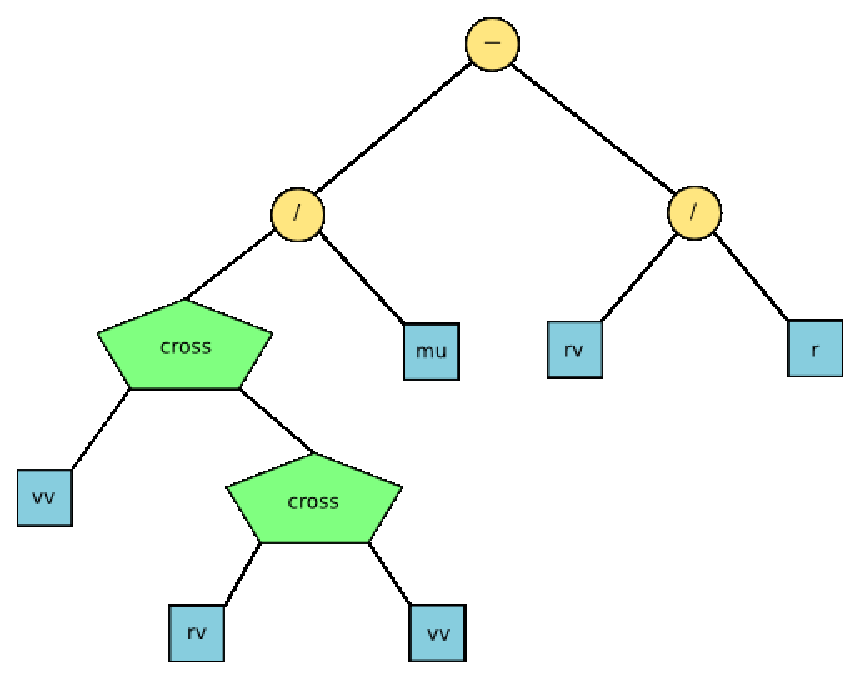
\includegraphics[scale=0.5]{Images/CrossMathTree.eps}
\caption{\label{figure:TwoFunMathTree}A MathTree with Two Function Calls.}
\end{center}
\end{figure}

\noindent Once this command has been built, the state of the system can be tabulated as in
Tables~\ref{table:EngineStatusWithCross} and~\ref{table:FunctionStatusWithCross}.

\begin{center}
\tablecaption{\label{table:EngineStatusWithCross}Status after Parsing the Assignment Line containing
Two Calls to the cross Function}
\tablefirsthead{\hline
\multicolumn{2}{|c|}{\textbf{Configuration}} &
\multirow{2}{1in}{\textbf{MCS}} &
\multirow{2}{*}{\textbf{Interpreter Mode}} &
\multirow{2}{*}{\textbf{Sandbox}} \\
\multicolumn{1}{|c}{\textit{Type}} & \multicolumn{1}{c|}{\textit{Name}} & & & \\
\hline
}
\tablehead{
\hline
\multicolumn{5}{|r|}{\begin{small}\textit{Continued from previous page}\end{small}}\\
\hline
\multicolumn{2}{|c|}{\textbf{Configuration}} &
\multirow{2}{1in}{\textbf{MCS}} &
\multirow{2}{*}{\textbf{Interpreter Mode}} &
\multirow{2}{*}{\textbf{Sandbox}} \\
\multicolumn{1}{|c}{\textit{Type}} & \multicolumn{1}{c|}{\textit{Name}} & & & \\
\hline }
\tabletail{\hline
\multicolumn{5}{|r|}{\begin{small}\textit{Continued on next page}\end{small}}\\ \hline }
\tablelasttail{\hline}
\begin{supertabular}{|l l|l|l|l|}
Spacecraft & Sat & While & Command & Idle\\
ForceModel & Prop\_FModel & +-- Propagate & & \\
Propagator & Prop & +-- CallFunction & & \\
Variable & SMA & +-- Assignment & & \\
... & ... & +-- Assignment & & \\
Array & nv & +-- Assignment & & \\
ReportFile & Cart2KepConvert & & & \\
GmatFunction & LoadCartState & & & \\
GmatFunction & cross & & & \\
\end{supertabular}
\end{center}

\noindent and

\begin{center}
\begin{small}
\tablecaption{\label{table:FunctionStatusWithCross}Function Properties after Parsing the cross
Assignment Line}
\tablefirsthead{\hline
\multirow{2}{*}{\textbf{Function}} &
\multirow{2}{*}{\textbf{Caller}} &
\multicolumn{3}{c|}{\textbf{Function Manager}} & \multicolumn{3}{c|}{\textbf{Function Attributes}}
\\
\cline{3-8}
 & & inputs, outputs & Function Object Store & Global Object Store &
inputs & outputs & FCS\\
\hline
}
\tablehead{
\hline \multicolumn{8}{|r|}{\begin{small}\textit{Continued from previous page}\end{small}}\\
\hline
\multirow{2}{*}{\textbf{Function}} &
\multirow{2}{*}{\textbf{Caller}} &
& \multicolumn{3}{c|}{\textbf{Function Manager}} &
\multicolumn{3}{c|}{\textbf{Function Attributes}}
\\
\cline{3-8}
 & & inputs, outputs & Function Object Store & Global Object Store & inputs & outputs & FCS\\
\hline
}
\tabletail{\hline
\multicolumn{8}{|r|}{\begin{small}\textit{Continued on next page}\end{small}}\\ \hline }
\tablelasttail{\hline}
\begin{supertabular}{|l|l|m{0.56in}|m{0.55in}|m{0.55in}|m{0.55in}|m{0.55in}|m{0.55in}|}
LoadCartState & CallFunction & Names set & Empty & NULL & Empty & Empty & Empty\\
cross & Function\-Runner & Names set & Empty & NULL & Empty & Empty & Empty\\
\end{supertabular}
\end{small}
\end{center}

There are two FunctionRunner nodes in the MathTree shown in Figure~\ref{figure:TwoFunMathTree}. 
Each one has its own FunctionManager.  The inputs and outputs StringArrays have the following values
for these FunctionManagers:

\begin{itemize}
\item Inner FunctionRunner MathNode
\end{itemize}

\begin{quote}
\begin{verbatim}
inputNames = {"rv", "vv"}
outputNames = {""}
\end{verbatim}
\end{quote}

\begin{itemize}
\item Outer FunctionRunner MathNode
\end{itemize}

\begin{quote}
\begin{verbatim}
inputNames = {"vv", ""}
outputNames = {""}
\end{verbatim}
\end{quote}

\noindent Note that at this point in the process, the unnamed arguments are marked using empty
strings in the StringArrays.  This is a general feature of the argument arrays generated in a
FunctionManager associated with a FunctionRunner: empty strings are used to indicate arguments that
must exist, but that do not have names that can be looked up in the object stores.  In general,
these empty strings indicate either output data or results that come from lower calculations
performed in the MathTree.

The next script line,

\begin{quote}
\begin{verbatim}
[ECC] = magnitude(ev);
\end{verbatim}
\end{quote}

\noindent builds another function call using a CallFunction, this time to the magnitude function. 
The resulting attributes are shown in Tables~\ref{table:EngineStatusWithMagnitude}
and~\ref{table:FunctionStatusWithMagnitude}.

\begin{center}
\tablecaption{\label{table:EngineStatusWithMagnitude}Status after Parsing the Call to the magnitude
Function}
\tablefirsthead{\hline
\multicolumn{2}{|c|}{\textbf{Configuration}} &
\multirow{2}{*}{\textbf{MCS}} &
\multirow{2}{*}{\textbf{Interpreter Mode}} &
\multirow{2}{*}{\textbf{Sandbox}} \\
\multicolumn{1}{|c}{\textit{Type}} & \multicolumn{1}{c|}{\textit{Name}} & & & \\
\hline
}
\tablehead{
\hline
\multicolumn{5}{|r|}{\begin{small}\textit{Continued from previous page}\end{small}}\\
\hline
\multicolumn{2}{|c|}{\textbf{Configuration}} &
\multirow{2}{*}{\textbf{MCS}} &
\multirow{2}{*}{\textbf{Interpreter Mode}} &
\multirow{2}{*}{\textbf{Sandbox}} \\
\multicolumn{1}{|c}{\textit{Type}} & \multicolumn{1}{c|}{\textit{Name}} & & & \\
\hline }
\tabletail{\hline
\multicolumn{5}{|r|}{\begin{small}\textit{Continued on next page}\end{small}}\\ \hline }
\tablelasttail{\hline}
\begin{supertabular}{|l l|l|l|l|}
Spacecraft & Sat & While & Command & Idle\\
ForceModel & Prop\_FModel & +-- Propagate & & \\
Propagator & Prop & +-- CallFunction & & \\
Variable & SMA & +-- Assignment & & \\
... & ... & +-- Assignment & & \\
Array & nv & +-- Assignment & & \\
ReportFile & Cart2KepConvert & +-- CallFunction & & \\
GmatFunction & LoadCartState & & & \\
GmatFunction & cross & & & \\
GmatFunction & magnitude & & & \\
\end{supertabular}
\end{center}

\noindent and

\begin{center}
\begin{small}
\tablecaption{\label{table:FunctionStatusWithMagnitude}Function Properties after Parsing the
magnitude Line}
\tablefirsthead{\hline
\multirow{2}{*}{\textbf{Function}} &
\multirow{2}{*}{\textbf{Caller}} &
\multicolumn{3}{c|}{\textbf{Function Manager}} & \multicolumn{3}{c|}{\textbf{Function Attributes}}
\\
\cline{3-8}
 & & inputs, outputs & Function Object Store & Global Object Store &
inputs & outputs & FCS\\
\hline
}
\tablehead{
\hline \multicolumn{8}{|r|}{\begin{small}\textit{Continued from previous page}\end{small}}\\
\hline
\multirow{2}{*}{\textbf{Function}} &
\multirow{2}{*}{\textbf{Caller}} &
\multicolumn{3}{c|}{\textbf{Function Manager}} &
\multicolumn{3}{c|}{\textbf{Function Attributes}}
\\
\cline{3-8}
 & & inputs, outputs & Function Object Store & Global Object Store & inputs & outputs & FCS\\
\hline
}
\tabletail{\hline
\multicolumn{8}{|r|}{\begin{small}\textit{Continued on next page}\end{small}}\\ \hline }
\tablelasttail{\hline}
\begin{supertabular}{|l|l|m{0.56in}|m{0.55in}|m{0.55in}|m{0.55in}|m{0.55in}|m{0.55in}|}
LoadCartState & CallFunction & Names set & Empty & NULL & Empty & Empty & Empty\\
cross & Function\-Runner & Names set & Empty & NULL & Empty & Empty & Empty\\
magnitude & CallFunction & Names set & Empty & NULL & Empty & Empty & Empty\\
\end{supertabular}
\end{small}
\end{center}

This process continues through the remaining lines of the script:

\begin{quote}
\begin{verbatim}
   nv(1,1)  =  x*vz-z*vx;
   nv(2,1)  =  y*vz-z*vy;
   nv(3,1)  =  0;
   [n] = magnitude(nv);
   RAAN = acos( nv(1,1)/n );
   If nv(2,1) < 0;
      RAAN = (pi2 - RAAN) / d2r;
   EndIf;

   SMAError  = Sat.SMA - SMA;
   ECCError  = Sat.ECC - ECC;
   RAANError = Sat.RAAN - RAAN;

   Report Cart2KepConvert Sat.SMA SMA SMAError ...
      Sat.ECC ECC ECCError Sat.RAAN RAAN RAANError;
EndWhile
\end{verbatim}
\end{quote}

\noindent The only line that calls a GMAT function here is the fourth line, a CallFunction command
that again calls the magnitude function.  At the end of parsing, our tables of object properties
look like this:

\begin{center}
\tablecaption{\label{table:EngineStatusAfterParsing}Status after Parsing the Script}
\tablefirsthead{\hline
\multicolumn{2}{|c|}{\textbf{Configuration}} &
\multirow{2}{*}{\textbf{MCS}} &
\multirow{2}{*}{\textbf{Interpreter Mode}} &
\multirow{2}{*}{\textbf{Sandbox}} \\
\multicolumn{1}{|c}{\textit{Type}} & \multicolumn{1}{c|}{\textit{Name}} & & & \\
\hline
}
\tablehead{
\hline
\multicolumn{5}{|r|}{\begin{small}\textit{Continued from previous page}\end{small}}\\
\hline
\multicolumn{2}{|c|}{\textbf{Configuration}} &
\multirow{2}{*}{\textbf{MCS}} &
\multirow{2}{*}{\textbf{Interpreter Mode}} &
\multirow{2}{*}{\textbf{Sandbox}} \\
\multicolumn{1}{|c}{\textit{Type}} & \multicolumn{1}{c|}{\textit{Name}} & & & \\
\hline }
\tabletail{\hline
\multicolumn{5}{|r|}{\begin{small}\textit{Continued on next page}\end{small}}\\ \hline }
\tablelasttail{\hline}
\begin{supertabular}{|l l|l|l|l|}
Spacecraft & Sat & While & Command & Idle\\
ForceModel & Prop\_FModel & +-- Propagate & & \\
Propagator & Prop & +-- CallFunction & & \\
Variable & SMA & +-- Assignment & & \\
Variable & ECC & +-- Assignment & & \\
Variable & RAAN & +-- Assignment & & \\
Variable & r & +-- CallFunction & & \\
Variable & v & +-- Assignment & & \\
Variable & pi2 & +-- Assignment & & \\
Variable & mu & +-- Assignment & & \\
Variable & d2r & +-- CallFunction & & \\
Variable & Energy & +-- Assignment & & \\
Variable & SMAError & +-- If & & \\
Variable & ECCError & +--+-- Assignment & & \\
Variable & RAANError & +-- EndIf & & \\
Array & rv & +-- Assignment & & \\
Array & vv & +-- Assignment & & \\
Array & ev & +-- Assignment & & \\
Array & nv & +-- Report & & \\
ReportFile & Cart2KepConvert & EndWhile & & \\
GmatFunction & LoadCartState & & & \\
GmatFunction & cross & & & \\
GmatFunction & magnitude & & & \\
\end{supertabular}
\end{center}

\noindent and

\begin{center}
\begin{small}
\tablecaption{\label{table:FunctionStatusAfterParsing}Function Properties after Parsing the Script}
\tablefirsthead{\hline
\multirow{2}{*}{\textbf{Function}} &
\multirow{2}{*}{\textbf{Caller}} &
\multicolumn{3}{c|}{\textbf{Function Manager}} & \multicolumn{3}{c|}{\textbf{Function Attributes}}
\\
\cline{3-8}
 & & inputs, outputs & Function Object Store & Global Object Store &
inputs & outputs & FCS\\
\hline
}
\tablehead{
\hline \multicolumn{8}{|r|}{\begin{small}\textit{Continued from previous page}\end{small}}\\
\hline
\multirow{2}{*}{\textbf{Function}} &
\multirow{2}{*}{\textbf{Caller}} &
\multicolumn{3}{c|}{\textbf{Function Manager}} &
\multicolumn{3}{c|}{\textbf{Function Attributes}}
\\
\cline{3-8}
 & & inputs, outputs & Function Object Store & Global Object Store & inputs & outputs & FCS\\
\hline
}
\tabletail{\hline
\multicolumn{8}{|r|}{\begin{small}\textit{Continued on next page}\end{small}}\\ \hline }
\tablelasttail{\hline}
\begin{supertabular}{|l|l|m{0.56in}|m{0.55in}|m{0.55in}|m{0.55in}|m{0.55in}|m{0.55in}|}
LoadCartState & CallFunction & Names set & Empty & NULL & Empty & Empty & Empty\\
cross & Function\-Runner & Names set & Empty & NULL & Empty & Empty & Empty\\
magnitude & CallFunction & Names set & Empty & NULL & Empty & Empty & Empty\\
\end{supertabular}
\end{small}
\end{center}

At this point in the process, the Configuration and Mission Control Sequence have been populated,
and three GMAT functions have been identified but not yet located.  The ScriptInterpreter has
finished parsing the script, but has not yet made its final pass through the objects created during
parsing.

During the final pass, object pointers and references are set and validated.  the ScriptInterpreter
uses the final pass to locate the function files for all of the  GmatFunction objects built during
parsing.  The path to each function is set at this time.  The ScriptInterpreter makes a call,
through the Moderator, and locates the function file on the GmatFunctionPath.  The file must be
named identically to the name of the function, with a file extension of ``.gmf'' -- so, for example,
the function file for the magnitude function must be named  ``magnitude.gmf''.  These file names
are case sensitive; a file named ``Magnitude.gmf'' will not match the ``magnitude'' function.  If
there is no matching file for the function, the ScriptInterpreter throws an exception.

Once this final pass is complete, script parsing has finished, and the ScriptInterpreter returns to
an idle state.  The steps followed to parse the Mission Control Sequence, described above, give GMAT
enough information to fully populate the GUI so that it can present users with a view of the mission
contained in the script.  The GUI includes entries for each of the functions in the main script,
and displays these functions along with all of the other configured objects on the Resource tree.

\subsubsection{Initialization in the Sandbox}

\begin{figure}
\begin{center}
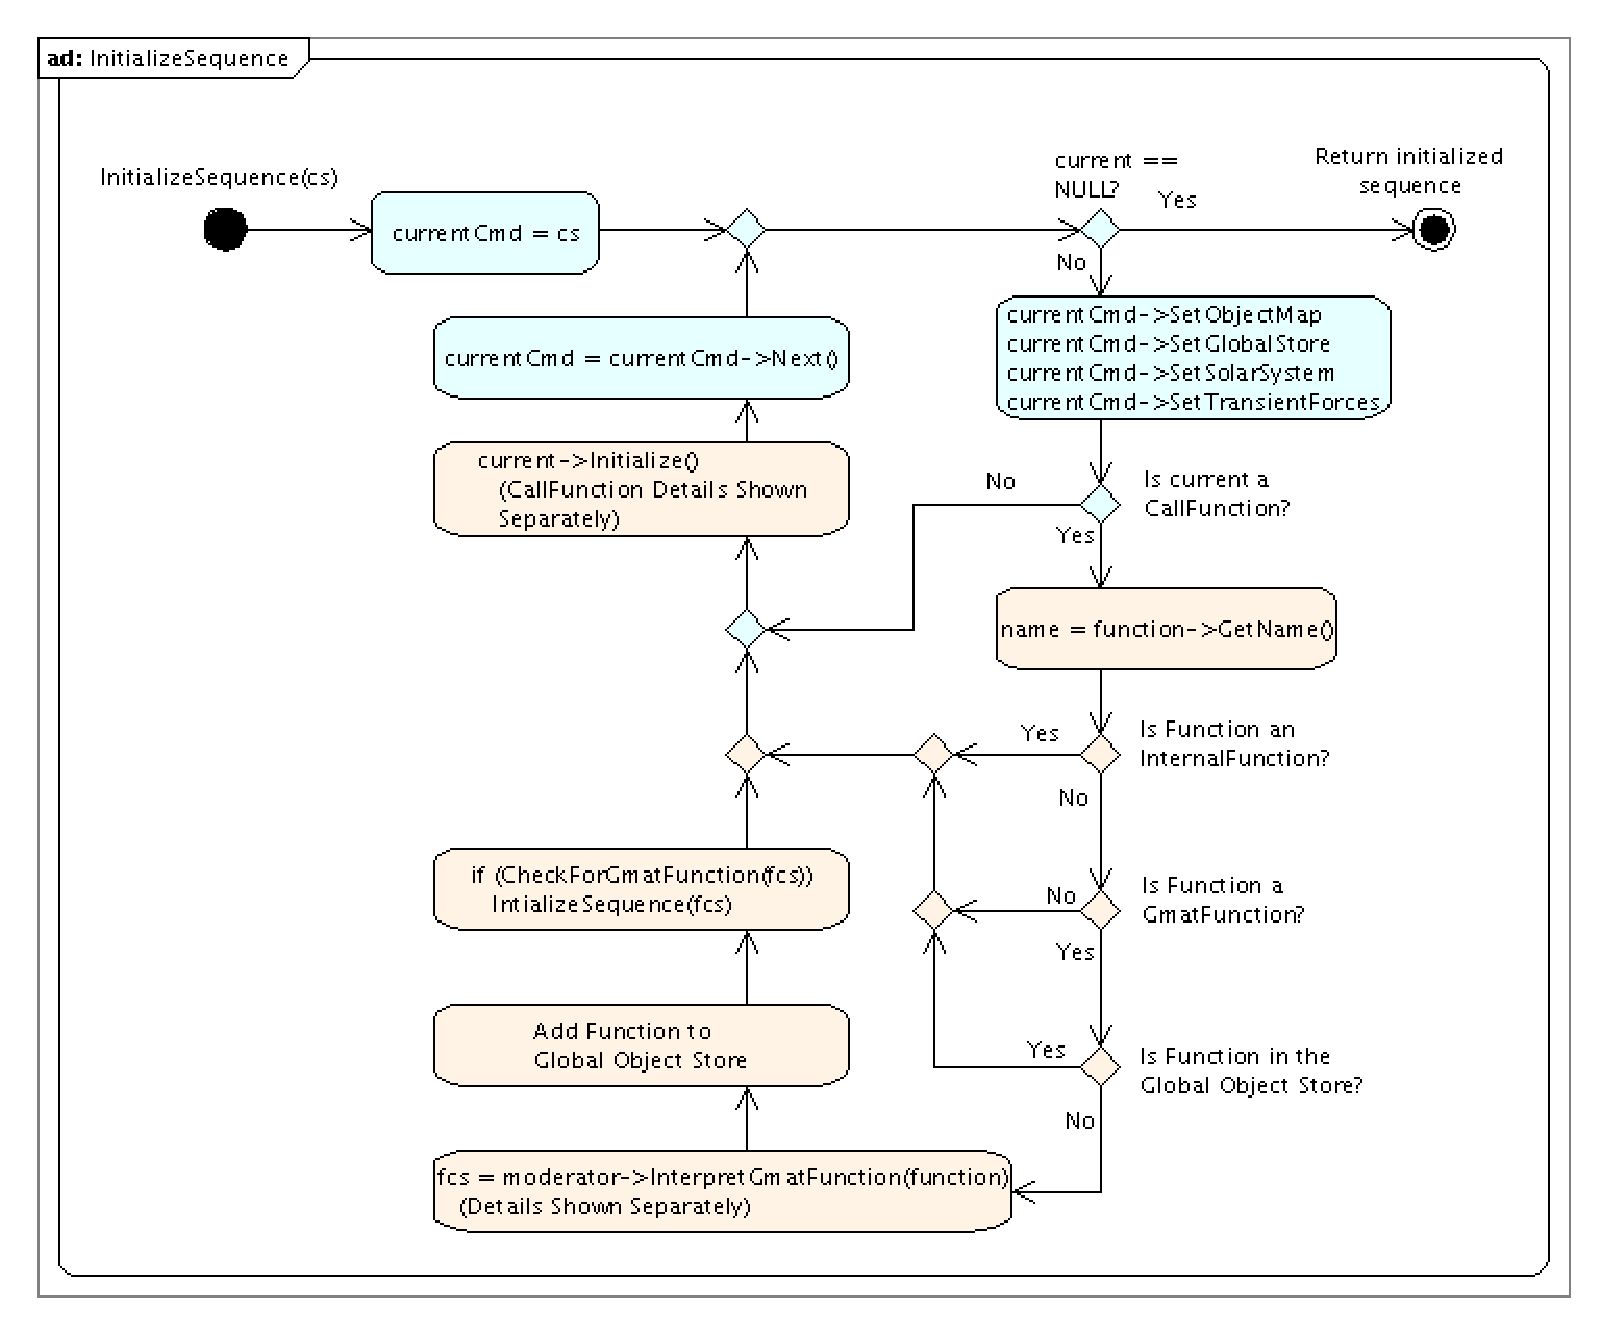
\includegraphics[scale=0.5]{Images/InitializeSequence.eps}
\caption{\label{figure:InitializeControlFunctionChapter}Initializing a Control Sequence}
\end{center}
\end{figure}

At this point, GMAT knows about the functions described in the Mission Control Sequence, but has not
yet constructed any of these functions.  That step is performed when the mission is passed into the
Sandbox and initialized.  The basic initialization process is described in
Chapters~\ref{chapter:TopLevel} and~\ref{chapter:Sandbox}.  The process followed can be described in
four stages:

\begin{enumerate}
\item \textbf{Population}: The objects in GMAT's configuration are cloned into the Sandbox Object
Map, and the Mission Control Sequence is set.
\item \textbf{Object Initialization}: The objects in the Sandbox Object Map are initialized.
\item \textbf{Global Object Management}: Objects that have their isGlobal flag set are moved
into the Global Object Store.
\item \textbf{Command Initialization}: The Mission Control Sequence is initialized.
\end{enumerate}

Outside of the cloning process, the GMAT function objects are not affected by the first two of these
steps.  Figure~\ref{figure:InitializeControlFunctionChapter}\footnote{This figure needs some
modification based on the text in the rest of this document.}, copied from
Chapter~\ref{chapter:Sandbox}, shows the process followed in the fourth step to initialize the
Mission Control Sequence.

Before going into the details of Figure~\ref{figure:InitializeControlFunctionChapter}, I'll describe
the activities performed in the first two steps.

\paragraph{Initialization Step 1: Passing Objects to the Sandbox}  The first step in initialization
is cloning the objects in the configuration into the Sandbox.  At the start of this step, the system
status looks like Table~\ref{table:EngineStatusAtInitStart}.  The Interpreter subsystem will not
play a role in this part of the initialization process -- the Interpreters remain idle -- so I will
remove that column for the time being in subsequent tables.

One feature of GMAT's design that can be overlooked is that there is a separate Mission Control
Sequence for each Sandbox, and there is a one-to-one relationship between the Mission Control
Sequences and the Sandbox instances.  What that means for this discussion is that the Mission
Control Sequence shown in the table already belongs to the Sandbox shown there.  The Mission Control
Sequence is not cloned into the Sandbox\footnote{This relationship between the Mission Control
Sequences and the array of Sandboxes is managed in the Moderator.  The behavior described here is
the default behavior, and is the behavior used in current implementations of GMAT.  Implementations
that use multiple Sandboxes -- particularly when used in a distributed manner -- will implement a
different relationship between the Mission Control Sequence viewed by the user and the Mission
Control Sequences in the Sandboxes.}.

\begin{center}
\tablecaption{\label{table:EngineStatusAtInitStart}Status Immediately Before Initialization Starts}
\tablefirsthead{\hline
\multicolumn{2}{|c|}{\textbf{Configuration}} &
\multirow{2}{*}{\textbf{MCS}} &
\multirow{2}{*}{\textbf{Interpreter Mode}} &
\multirow{2}{*}{\textbf{Sandbox}} \\
\multicolumn{1}{|c}{\textit{Type}} & \multicolumn{1}{c|}{\textit{Name}} & & & \\
\hline
}
\tablehead{
\hline
\multicolumn{5}{|r|}{\begin{small}\textit{Continued from previous page}\end{small}}\\
\hline
\multicolumn{2}{|c|}{\textbf{Configuration}} &
\multirow{2}{*}{\textbf{MCS}} &
\multirow{2}{*}{\textbf{Interpreter Mode}} &
\multirow{2}{*}{\textbf{Sandbox}} \\
\multicolumn{1}{|c}{\textit{Type}} & \multicolumn{1}{c|}{\textit{Name}} & & & \\
\hline }
\tabletail{\hline
\multicolumn{5}{|r|}{\begin{small}\textit{Continued on next page}\end{small}}\\ \hline }
\tablelasttail{\hline}
\begin{supertabular}{|l l|l|l|l|}
Spacecraft & Sat & While & Idle & Idle, Sandbox Object\\
ForceModel & Prop\_FModel & +-- Propagate & & Map is Empty \\
Propagator & Prop & +-- CallFunction & & \\
Variable & SMA & +-- Assignment & & \\
Variable & ECC & +-- Assignment & & \\
Variable & RAAN & +-- Assignment & & \\
Variable & r & +-- CallFunction & & \\
Variable & v & +-- Assignment & & \\
Variable & pi2 & +-- Assignment & & \\
Variable & mu & +-- Assignment & & \\
Variable & d2r & +-- CallFunction & & \\
Variable & Energy & +-- Assignment & & \\
Variable & SMAError & +-- If & & \\
Variable & ECCError & +--+-- Assignment & & \\
Variable & RAANError & +-- EndIf & & \\
Array & rv & +-- Assignment & & \\
Array & vv & +-- Assignment & & \\
Array & ev & +-- Assignment & & \\
Array & nv & +-- Report & & \\
ReportFile & Cart2KepConvert & EndWhile & & \\
GmatFunction & LoadCartState & & & \\
GmatFunction & cross & & & \\
GmatFunction & magnitude & & & \\
\end{supertabular}
\end{center}

The objects in the configuration, on the other hand, are contained in GMAT's engine, outside of the
Sandbox.  The Moderator accesses these configured objects by type, and passes each into the Sandbox
for use in the mission.  The Sandbox makes copies of these objects using the object's Clone()
method.  These clones are stored in the Sandbox Object Map.  The clones contain identical data to
the objects in the configuration; making clones at this stage preserves the user's settings on the
configured objects while providing working copies that are used to run the mission.

Table\ref{table:EngineStatusAfterConfigCloning} shows the status of the system after the Moderator
has passed the objects into the Sandbox.  The Sandbox Object Map is a mapping between a text name
and a pointer to the associated object.  Since the map is from the name to the object, the Sandbox
Object Map in the table lists the name first.

\begin{center}
\tablecaption{\label{table:EngineStatusAfterConfigCloning}Status Immediately After Cloning into the
Sandbox}
\tablefirsthead{\hline
\multicolumn{2}{|c|}{\textbf{Configuration}} &
\multicolumn{3}{c|}{\textbf{Sandbox}} \\
\hline
\multicolumn{1}{|c}{\textit{Scripted}} &
\multicolumn{1}{c|}{\multirow{2}{*}{\textit{Name}}} &
\multicolumn{1}{c|}{\multirow{2}{*}{\textbf{MCS}}} &
\multicolumn{2}{c|}{\textbf{Sandbox Object Map}} \\
\cline{4-5}
\multicolumn{1}{|c}{\textit{Type}}& & & \textit{Name} & \textit{Type} \\
\hline
}
\tablehead{
\hline
\multicolumn{5}{|r|}{\begin{small}\textit{Continued from previous page}\end{small}}\\
\hline
\multicolumn{2}{|c|}{\textbf{Configuration}} &
\multicolumn{3}{c|}{\textbf{Sandbox}} \\
\hline
\multicolumn{1}{|c}{\textit{Scripted}} &
\multicolumn{1}{c|}{\multirow{2}{*}{\textit{Name}}} &
\multicolumn{1}{c|}{\multirow{2}{*}{\textbf{MCS}}} &
\multicolumn{2}{c|}{\textbf{Sandbox Object Map}} \\
\cline{4-5}
\multicolumn{1}{|c}{\textit{Type}}& & & \textit{Name} & \textit{Type} \\
\hline }
\tabletail{\hline
\multicolumn{5}{|r|}{\begin{small}\textit{Continued on next page}\end{small}}\\ \hline }
\tablelasttail{\hline}
\begin{supertabular}{|l l|l|l|l|}
Spacecraft & Sat & While & Sat & Spacecraft*\\
ForceModel & Prop\_FModel & +-- Propagate & Prop\_FModel & ForceModel* \\
Propagator & Prop & +-- CallFunction & Prop & PropSetup*\\
Variable & SMA & +-- Assignment & SMA & Variable* \\
Variable & ECC & +-- Assignment & ECC & Variable* \\
Variable & RAAN & +-- Assignment & RAAN & Variable* \\
Variable & r & +-- CallFunction & r & Variable* \\
Variable & v & +-- Assignment & v & Variable* \\
Variable & pi2 & +-- Assignment & pi2 & Variable* \\
Variable & mu & +-- Assignment & mu & Variable* \\
Variable & d2r & +-- CallFunction & d2r & Variable* \\
Variable & Energy & +-- Assignment & Energy & Variable* \\
Variable & SMAError & +-- If & SMAError & Variable* \\
Variable & ECCError & +--+-- Assignment & ECCError & Variable* \\
Variable & RAANError & +-- EndIf & RAANError & Variable* \\
Array & rv & +-- Assignment & rv & Array* \\
Array & vv & +-- Assignment & vv & Array* \\
Array & ev & +-- Assignment & ev & Array* \\
Array & nv & +-- Report & nv & Array* \\
ReportFile & Cart2KepConvert & EndWhile & Cart2KepConvert & ReportFile* \\
GmatFunction & LoadCartState & & LoadCartState & GmatFunction* \\
GmatFunction & cross & & cross & GmatFunction* \\
GmatFunction & magnitude & & magnitude & GmatFunction* \\
CoordinateSystem\footnote & EarthMJ2000Eq & & EarthMJ2000Eq &
CoordinateSystem* \\
CoordinateSystem & EarthMJ2000Ec & & EarthMJ2000Ec & CoordinateSystem* \\
CoordinateSystem & EarthFixed & & EarthFixed & CoordinateSystem* \\
\end{supertabular}
\end{center}
\footnotetext{The 3 coordinate systems listed at the end of the configuration table are
automatically created by the Moderator.}

Once the Moderator has passed the Configuration into the Sandbox, the mission run no longer depends
on the Configuration.  For that reason, most of the tables shown in the rest of this document will
not include a list of the contents of the configuration.  If needed, the Configuration will be
displayed separately.

\paragraph{Initialization Step 2: Object Initialization} Now that the Sandbox has been populated
with the configured objects and the Mission Control Sequence, the Moderator can pass control to the
Sandbox to continue the initialization process.  This hand off is made through a call to the
Sandbox::Initialize() method.  The Sandbox initializes objects in the following order:

\begin{enumerate}
\item CoordinateSystem
\item Spacecraft
\item All others except Parameters and Subscribers
\item System Parameters
\item Other Parameters
\item Subscribers
\end{enumerate}

\noindent The initialization of these objects follows this basic algorithm:

\begin{itemize}
\item Send the Sandbox's solar system to the object
\item Set pointers for all of objects referenced by this object
\item Call the object's Initialize() method
\end{itemize}

\noindent The basic initialization for Function objects are part of element 3 in the list above.  At
that point in the initialization process, the Function objects are not yet populated, so this step
does not perform any substantive action.  The Sandbox checks each GmatFunction to ensure that the
path to the function file is not empty as part of this initialization.

\paragraph{\label{section:GlobalObjectManagement}Initialization Step 3: Global Object Management}
Once the objects in the Sandbox Object Map are initialized, the objects flagged as global objects
are moved from the Sandbox Object Map into the Global Object Store.  The Sandbox does this by
checking the object's isGlobal flag, a new attribute of the GmatBase class added for global object
management.

Some object types are automatically marked as global objects.  All instances of the PropSetup class,
Function classes, and coordinate system classes fall into this category, and are built with the
isGlobal flag set.

\paragraph{Initialization Step 4: Control Sequence Initialization}  The final step in Sandbox
initialization is initialization of the Mission Control Sequence.  This step in the initialization
process includes construction of the Function Control Sequences, and does the first portion of
initialization that is needed before the Function Control Sequence can be executed.  At this stage
in the initialization process, the Global Object Store contains clones of all of the configured
objects marked as globals, the Sandbox Object Map contains clones of all other configured objects,
and the GmatFunction objects know the locations of the function files.  The Function Control
Sequences are all empty, and the system has not identified any functions called from inside of
functions that are not also called in the Mission Control Sequence. The objects in the Sandbox
Object Map have the connections to referenced objects set, and are ready for use in the Mission
Control Sequence.

So far, we have encountered three GmatFunctions, shown in
Table~\ref{table:FunctionStatusCSInitStart} with their data structures:

\begin{center}
\tablecaption{\label{table:FunctionStatusCSInitStart}GmatFunction Status at the Start of
Control Sequence Initialization}
\tablefirsthead{
\hline
%\color{blue}
\multicolumn{1}{|p{0.9in}|}{\textbf{Function}} &
\multicolumn{1}{m{0.8in}|}{\textbf{Function Object Store}} &
\multicolumn{1}{m{0.7in}|}{\textbf{Global Object Store}} &
\multicolumn{1}{m{0.7in}|}{\textbf{inputs}} &
\multicolumn{1}{m{0.7in}|}{\textbf{outputs}} &
\multicolumn{1}{m{0.8in}|}{\textbf{Function Control Sequence}} &
\multicolumn{1}{m{0.7in}|}{\textbf{Call Stack}} \\
%\color{black}
\hline
}
\tablehead{
% \hline
% \multicolumn{7}{|r|}{\begin{small}\textit{Continued from previous page}\end{small}}\\
% \hline
% %\color{blue}
% \multicolumn{1}{|m{0.9in}|}{\textbf{Function}} &
% \multicolumn{1}{m{0.8in}|}{\textbf{Function Object Store}} &
% \multicolumn{1}{m{0.7in}|}{\textbf{Global Object Store}} &
% \multicolumn{1}{m{0.7in}|}{\textbf{inputs}} &
% \multicolumn{1}{m{0.7in}|}{\textbf{outputs}} &
% \multicolumn{1}{m{0.8in}|}{\textbf{Function Control Sequence}} &
% \multicolumn{1}{m{0.7in}|}{\textbf{Call Stack}} \\
% %\color{black}
% \hline
}
\tabletail{
% \hline
% \multicolumn{7}{|r|}{\begin{small}\textit{Continued on next page}\end{small}}\\ \hline
}
\tablelasttail{\hline}
\begin{supertabular}{|m{0.9in}|m{0.8in}|m{0.7in}|m{0.7in}|m{0.7in}|m{0.8in}|m{0.7in}|}
LoadCartState & empty & NULL & empty & empty & empty & empty\\ \hline
cross & empty & NULL & empty & empty & empty & empty\\ \hline
magnitude & empty & NULL & empty & empty & empty & empty\\ \hline
\end{supertabular}
\end{center}

\noindent As we will see, the call stack, implemented as the ``objectStack'' attribute in the
GmatFunction class, remains empty throughout the initialization process.

The Sandbox initialized the Mission Control Sequence by walking through the list of commands in the
sequence, and performing the following tasks on each:

\begin{itemize}
\item Send the pointers to the Sandbox Object Map and the Global Object Map to the command
\item Set the solar system pointer for the command
\item Set the transient force vector for the command
\item If the command uses a GmatFunction, build that function as described below
\item Call the command's Initialize() method
\end{itemize}
\noindent In order to see how these actions work with GmatFunctions, we'll continue walking through
the sample script.  For clarity's sake, it is useful to have a complete picture of the contents of
the Mission Control Sequence.  The Mission Control Sequence, listed by node type and script line,
and numbered for reference, can be written like this:

\begin{center}
\tablefirsthead{}
\tablehead{}
\tabletail{}
\tablelasttail{}
\begin{supertabular}{lllp{4in}}
\begin{footnotesize}1\end{footnotesize} & While & & \texttt{While Sat.ElapsedDays < 1}\\
\begin{footnotesize}2\end{footnotesize} & Propagate & & \texttt{\ \ \ Propagate Prop(Sat)}\\
\begin{footnotesize}3\end{footnotesize} & CallFunction & & \texttt{\ \ \ [rv, vv, r, v] =
LoadCartState(Sat);}\\
\begin{footnotesize}4\end{footnotesize} & Assignment & & \texttt{\ \ \ Energy = v\^{}2/2 - mu/r;}\\
\begin{footnotesize}5\end{footnotesize} & Assignment & & \texttt{\ \ \ SMA = -mu/2/Energy;}\\
\begin{footnotesize}6\end{footnotesize} & Assignment & & \texttt{\ \ \ ev = cross(vv,cross(rv,
vv))/mu - rv/r;}\\
\begin{footnotesize}7\end{footnotesize} & CallFunction & & \texttt{\ \ \ [ECC] = magnitude(ev);}\\
\begin{footnotesize}8\end{footnotesize} & Assignment & & \texttt{\ \ \ nv(1,1)  =  x*vz-z*vx;}\\
\begin{footnotesize}9\end{footnotesize} & Assignment & & \texttt{\ \ \ nv(2,1)  =  y*vz-z*vy;}\\
\begin{footnotesize}10\end{footnotesize} & Assignment & & \texttt{\ \ \ nv(3,1)  =  0;}\\
\begin{footnotesize}11\end{footnotesize} & CallFunction & & \texttt{\ \ \ [n] = magnitude(nv);}\\
\begin{footnotesize}12\end{footnotesize} & Assignment & & \texttt{\ \ \ RAAN = acos( nv(1,1)/n );}\\
\begin{footnotesize}13\end{footnotesize} & If & & \texttt{\ \ \ If nv(2,1) < 0;}\\
\begin{footnotesize}14\end{footnotesize} & Assignment & & \texttt{\ \ \ \ \ \ RAAN = (pi2 - RAAN)
/ d2r;}\\
\begin{footnotesize}15\end{footnotesize} & EndIf & & \texttt{\ \ \ EndIf;}\\
\begin{footnotesize}16\end{footnotesize} & Assignment & & \texttt{\ \ \ SMAError  = Sat.SMA -
SMA;}\\
\begin{footnotesize}17\end{footnotesize} & Assignment & & \texttt{\ \ \ ECCError  = Sat.ECC -
ECC;}\\
\begin{footnotesize}18\end{footnotesize} & Assignment & & \texttt{\ \ \ RAANError = Sat.RAAN -
RAAN;}\\
\begin{footnotesize}19\end{footnotesize} & Report & & \texttt{\ \ \ Report Cart2KepConvert Sat.SMA
SMA SMAError ...}\\
& & & \ \ \ \ \ \ \ \ \texttt{Sat.ECC ECC ECCError Sat.RAAN RAAN RAANError}\\
\begin{footnotesize}20\end{footnotesize} & EndWhile & & \texttt{EndWhile}\\
\end{supertabular}
\end{center}

\noindent (The line of script associated with each node is shown on the right in this list.)

At the start of the Mission Control Sequence initialization, the Sandbox Object Map and Global
Object Store contain the following items:

\pagebreak 

\begin{center}
\tablecaption{\label{table:CSInitStartSandboxMaps}The Sandbox Maps}
\tablefirsthead{
\hline
\multicolumn{2}{|c|}{\textbf{Sandbox Object Map}} & \multicolumn{2}{c|}{\textbf{Global Object
Store}} \\
\hline
\multicolumn{1}{|c}{\textit{Name}} & \multicolumn{1}{c|}{\textit{Type}} &
\multicolumn{1}{c}{\textit{Name}} & \multicolumn{1}{c|}{\textit{Type}}\\
\hline
}
\tablehead{
\hline\multicolumn{4}{|r|}{\begin{small}\textit{Continued from previous page}\end{small}}\\
\hline
\multicolumn{2}{|c|}{\textbf{Sandbox Object Map}} & \multicolumn{2}{c|}{\textbf{Global Object
Store}} \\
\hline
\multicolumn{1}{|c}{\textit{Name}} & \multicolumn{1}{c|}{\textit{Type}} &
\multicolumn{1}{c}{\textit{Name}} & \multicolumn{1}{c|}{\textit{Type}}\\
\hline
}
\tabletail{\hline\multicolumn{4}{|r|}{\begin{small}\textit{Continued on next page}\end{small}}\\
\hline}
\tablelasttail{\hline}
\begin{supertabular}{|p{1.4in}p{1.4in}|p{1.4in}p{1.4in}|}
Sat & Spacecraft* & Prop & PropSetup* \\
Prop\_FModel & ForceModel* & EarthMJ2000Eq & CoordinateSystem* \\
Prop & PropSetup* & EarthMJ2000Ec & CoordinateSystem*\\
SMA & Variable* & EarthFixed & CoordinateSystem*\\
ECC & Variable* & LoadCartState & GmatFunction*\\
RAAN & Variable* & cross & GmatFunction*\\
r & Variable* & magnitude & GmatFunction*\\
v & Variable* & & \\
pi2 & Variable* & & \\
mu & Variable* & & \\
d2r & Variable* & & \\
Energy & Variable* & & \\
SMAError & Variable* & & \\
ECCError & Variable* & & \\
RAANError & Variable* & & \\
rv & Array* & & \\
vv & Array* & & \\
ev & Array* & & \\
nv & Array* & & \\
Cart2KepConvert & ReportFile* & & \\
LoadCartState & GmatFunction* & & \\
cross & GmatFunction* & & \\
magnitude & GmatFunction* & & \\
EarthMJ2000Eq & CoordinateSystem* & & \\
EarthMJ2000Ec & CoordinateSystem* & & \\
EarthFixed & CoordinateSystem* & & \\
\end{supertabular}
\end{center}

\noindent These maps stay the same until either a Global command is encountered or a Create command
is encountered that creates an object that is automatically global.

The steps listed above for command initialization are performed for the first two commands in the
list, items 1 and 2, without changing any of the object maps or function attributes.  Item 3:

\begin{quote}
\begin{verbatim}
[rv, vv, r, v] = LoadCartState(Sat);
\end{verbatim}
\end{quote}

\noindent is a CallFunction that initializes a GmatCommand, so we need to look more closely at the
initialization for this line.

The CallFunction at this point has a FunctionManager which contains the name of a GmatFunction
object and StringArrays for the inputs and outputs.  The StringArrays contain the following data:

\begin{quote}
\begin{verbatim}
inputNames = {"Sat"}
outputNames = {"rv", "vv", "r", "v"}
\end{verbatim}
\end{quote}

The Sandbox passes the pointers for the Sandbox Object Map and the Global Object Store to the
CallFunction command.  Once the CallFunction has received the Global Object Store, it uses that
mapping to locate the function needed by the Function Manager, and passes the pointer to that
function into the FunctionManager.  The FunctionManager determines the type of the function -- in
this example, the function is a GmatFunction.  The function attributes at this point are shown in
Table~\ref{table:GMFPostGOSSOM}.

\pagebreak 

\begin{center}
\tablefirsthead{
\hline
%\color{blue}
\multicolumn{1}{|p{0.9in}|}{\textbf{Function}} &
\multicolumn{1}{m{0.8in}|}{\textbf{Function Object Store}} &
\multicolumn{1}{m{0.7in}|}{\textbf{Global Object Store}} &
\multicolumn{1}{m{0.7in}|}{\textbf{inputs}} &
\multicolumn{1}{m{0.7in}|}{\textbf{outputs}} &
\multicolumn{1}{m{0.8in}|}{\textbf{Function Control Sequence}} &
\multicolumn{1}{m{0.7in}|}{\textbf{Call Stack}} \\
%\color{black}
\hline
}
\tablehead{
\hline
\multicolumn{7}{|r|}{\begin{small}\textit{Continued from previous page}\end{small}}\\
\hline
%\color{blue}
\multicolumn{1}{|m{0.9in}|}{\textbf{Function}} &
\multicolumn{1}{m{0.8in}|}{\textbf{Function Object Store}} &
\multicolumn{1}{m{0.7in}|}{\textbf{Global Object Store}} &
\multicolumn{1}{m{0.7in}|}{\textbf{inputs}} &
\multicolumn{1}{m{0.7in}|}{\textbf{outputs}} &
\multicolumn{1}{m{0.8in}|}{\textbf{Function Control Sequence}} &
\multicolumn{1}{m{0.7in}|}{\textbf{Call Stack}} \\
%\color{black}
\hline
}
\tabletail{
\hline
\multicolumn{7}{|r|}{\begin{small}\textit{Continued on next page}\end{small}}\\ \hline
}
\tablelasttail{\hline}
\tablecaption{\label{table:GMFPostGOSSOM}GmatFunction Status after Setting the GOS and SOM}
\begin{supertabular}{|m{0.9in}|m{0.8in}|m{0.7in}|m{0.7in}|m{0.7in}|m{0.8in}|m{0.7in}|}
\hline
LoadCartState & empty & Set & empty & empty & empty & empty\\\hline
cross & empty & NULL & empty & empty & empty & empty\\\hline
magnitude & empty & NULL & empty & empty & empty & empty\\\hline
\end{supertabular}
\end{center}

The Sandbox then passes in the pointers to the solar system and transient force vector, which the
CallFunction passes into the FunctionManager.  Since the function in the FunctionManager is a
GmatFunction, these pointers will be needed later in initialization and execution, so the
FunctionManager passes these pointers into the function for later use.  (If the function in the
FunctionManger was not a GmatFunction, the pointers would have been discarded.)

At this point, all of the items needed to build the Function Control Sequence exist.  The Sandbox
retrieves the pointer for the GmatFunction from the CallFunction command.  It checks to see if the
function's Function Control Sequence has been built.  If the Function Control Sequence is NULL, the
Sandbox calls the Moderator::InterpretGmatFunction() method to construct the Function Control
Sequence, which in turn calls the ScriptInterpreter::InterpretGmatFunction() method.  Both of these
calls take the function pointer as input arguments, so that the interpreter has the local Sandbox
instance of the GmatFunction that it uses to build the Function Control Sequence.  The
ScriptInterpreter::InterpretGmatFunction() method builds the Function Control Sequence and returns
it, through the Moderator, to the Sandbox.

The LoadCartState GmatFunction that is constructed here is built from this scripting:

\begin{quote}
\begin{verbatim}
function [rv, vv, r, v] = LoadCartState(Sat);

% This function fills some arrays and variables with
% Cartesian state data

Create Variable r v
Create Array rv[3,1] vv[3,1]

rv(1,1) = Sat.X;
rv(1,2) = Sat.Y;
rv(1,3) = Sat.Z;
vv(1,1) = Sat.VX;
vv(1,2) = Sat.VY;
vv(1,3) = Sat.VZ;

[r] = magnitude(rv);
[v] = magnitude(vv);
\end{verbatim}
\end{quote}

The process followed in the ScriptInterpreter::InterpretGmatFunction() method will be described
below.  Upon return from this function call, the functions contain the attributes shown in
Table~\ref{table:GMFPostLoadCartState}.

\pagebreak 

\begin{center}
\tablecaption{\label{table:GMFPostLoadCartState}GmatFunction Status after Building the LoadCartState
FCS}
\tablefirsthead{
\hline
%\color{blue}
\multicolumn{1}{|p{0.9in}|}{\textbf{Function}} &
\multicolumn{1}{m{0.7in}|}{\textbf{Function Object Store}} &
\multicolumn{1}{m{0.7in}|}{\textbf{Global Object Store}} &
\multicolumn{1}{m{0.75in}|}{\textbf{inputs}} &
\multicolumn{1}{m{0.75in}|}{\textbf{outputs}} &
\multicolumn{1}{m{0.8in}|}{\textbf{Function Control Sequence}} &
\multicolumn{1}{m{0.7in}|}{\textbf{Call Stack}} \\
%\color{black}
\hline
}
\tablehead{
% \hline
% \multicolumn{7}{|r|}{\begin{small}\textit{Continued from previous page}\end{small}}\\
% \hline
% %\color{blue}
% \multicolumn{1}{|m{0.9in}|}{\textbf{Function}} &
% \multicolumn{1}{m{0.7in}|}{\textbf{Function Object Store}} &
% \multicolumn{1}{m{0.7in}|}{\textbf{Global Object Store}} &
% \multicolumn{1}{m{0.75in}|}{\textbf{inputs}} &
% \multicolumn{1}{m{0.75in}|}{\textbf{outputs}} &
% \multicolumn{1}{m{0.8in}|}{\textbf{Function Control Sequence}} &
% \multicolumn{1}{m{0.7in}|}{\textbf{Call Stack}} \\
% %\color{black}
% \hline
}
\tabletail{
% \hline
% \multicolumn{7}{|r|}{\begin{small}\textit{Continued on next page}\end{small}}\\ \hline
}
\tablelasttail{\hline}
\begin{supertabular}{|p{0.9in}|p{0.7in}|p{0.7in}|p{0.75in}|p{0.75in}|p{0.8in}|p{0.7in}|}
\hline
\begin{small}LoadCartState\end{small} &
\begin{small}empty\end{small} &
\begin{small}Set\end{small} &
\begin{small}'Sat'->NULL\end{small} &
\begin{small}'rv'->NULL

'vv'->NULL

'r'->NULL

'v'->NULL\end{small} &
\begin{small}Create

Create

Assignment

Assignment

Assignment

Assignment

Assignment

Assignment

CallFunction

CallFunction\end{small} &
\begin{small}empty\end{small}\\
\hline
\begin{small}cross\end{small} & \begin{small}empty\end{small} &
\begin{small}NULL\end{small} & \begin{small}empty\end{small} &
\begin{small}empty\end{small} & \begin{small}empty\end{small} &
\begin{small}empty\end{small}\\\hline
\begin{small}magnitude\end{small} & \begin{small}empty\end{small} & \begin{small}NULL\end{small} &
\begin{small}empty\end{small} & \begin{small}empty\end{small} &
\begin{small}empty\end{small} & \begin{small}empty\end{small}\\
\hline
\end{supertabular}
\end{center}

The Sandbox then checks the Function Control Sequence generated in the ScriptInterpreter, and checks
to see if that sequence contains a GmatFunction.  If it does, then for each GmatFunction
encountered, the process is repeated.

The Sandbox checks the Function Control Sequence by starting at the first node, and checking each
Assignment and CallFunction command in that control sequence to see if it references a GmatFunction.
 Our example script does contain such a call to a GmatFunction -- it calls the magnitude function
twice, in the last two CallFunction commands in the Function Control Sequence.  Each of the
FunctionManagers associated with these CallFunction commands have StringArrays containing the names
of the input and output objects that will be used during execution -- more specifically, the
FunctionManager associated with the first CallFunction has these StringArrays:

\begin{quote}
\begin{verbatim}
inputNames = {"rv"}
outputNames = {"r"}
\end{verbatim}
\end{quote}

\noindent while the second has these:

\begin{quote}
\begin{verbatim}
inputNames = {"vv"}
outputNames = {"v"}
\end{verbatim}
\end{quote}

When the Sandbox detects the GmatFunction in the first CallFunction command, it performs the same
tasks as were performed on the CallFunction in the Mission Control Sequence -- more specifically:

\begin{enumerate}
\item The Sandbox passes the pointer for the Global Object Store to the CallFunction command.  (Note
that the Sandbox does not pass in the Sandbox Object Map; the Sandbox Object Map is only used in
commands in the Mission Control Sequence.)
\item Once the CallFunction has received the Global Object Store, it uses that mapping to locate the
function needed by the FunctionManager.
\begin{itemize}
\item If the function was found, the CallFunction passes the pointer to that function into the
FunctionManager
\item If the function was not found, the pointer referenced by the Function Manager remains NULL.
\end{itemize}
\item The FunctionManager determines the type of the function.  If the function is not a
GmatFunction, the process ends.
\item The Sandbox passes the pointers to the solar system and transient force vector to the
CallFunction, which passes them into the FunctionManager.
\item The FunctionManager passes these pointers into the function for later use.
\end{enumerate}

At this point, all of the items needed to build the nested Function Control Sequence exist. 
Returning to our example, the state of the function object attributes at this point is shown in
Table~\ref{table:GMFFirstNestedFunction}.

\begin{center}
\tablecaption{\label{table:GMFFirstNestedFunction}GmatFunction Status after Detecting the First
Nested
CallFunction}
\tablefirsthead{
\hline
%\color{blue}
\multicolumn{1}{|p{0.9in}|}{\textbf{Function}} &
\multicolumn{1}{m{0.7in}|}{\textbf{Function Object Store}} &
\multicolumn{1}{m{0.7in}|}{\textbf{Global Object Store}} &
\multicolumn{1}{m{0.75in}|}{\textbf{inputs}} &
\multicolumn{1}{m{0.75in}|}{\textbf{outputs}} &
\multicolumn{1}{m{0.8in}|}{\textbf{Function Control Sequence}} &
\multicolumn{1}{m{0.7in}|}{\textbf{Call Stack}} \\
%\color{black}
\hline
}
\tablehead{
% \hline
% \multicolumn{7}{|r|}{\begin{small}\textit{Continued from previous page}\end{small}}\\
% \hline
% %\color{blue}
% \multicolumn{1}{|m{0.9in}|}{\textbf{Function}} &
% \multicolumn{1}{m{0.7in}|}{\textbf{Function Object Store}} &
% \multicolumn{1}{m{0.7in}|}{\textbf{Global Object Store}} &
% \multicolumn{1}{m{0.75in}|}{\textbf{inputs}} &
% \multicolumn{1}{m{0.75in}|}{\textbf{outputs}} &
% \multicolumn{1}{m{0.8in}|}{\textbf{Function Control Sequence}} &
% \multicolumn{1}{m{0.7in}|}{\textbf{Call Stack}} \\
% %\color{black}
% \hline
}
\tabletail{
% \hline
% \multicolumn{7}{|r|}{\begin{small}\textit{Continued on next page}\end{small}}\\ \hline
}
\tablelasttail{\hline}
\begin{supertabular}{|p{0.9in}|p{0.7in}|p{0.7in}|p{0.75in}|p{0.75in}|p{0.8in}|p{0.7in}|}
\hline
\begin{small}LoadCartState\end{small} &
\begin{small}empty\end{small} &
\begin{small}Set\end{small} &
\begin{small}'Sat'->NULL\end{small} &
\begin{small}'rv'->NULL

'vv'->NULL

'r'->NULL

'v'->NULL\end{small} &
\begin{small}Create

Create

Assignment

Assignment

Assignment

Assignment

Assignment

Assignment

CallFunction

CallFunction\end{small} &
\begin{small}empty\end{small}\\
\hline
\begin{small}cross\end{small} & \begin{small}empty\end{small} &
\begin{small}NULL\end{small} & \begin{small}empty\end{small} &
\begin{small}empty\end{small} & \begin{small}empty\end{small} &
\begin{small}empty\end{small}\\\hline
\begin{small}magnitude\end{small} & \begin{small}empty\end{small} & \begin{small}Set\end{small} &
\begin{small}empty\end{small} & \begin{small}empty\end{small} &
\begin{small}empty\end{small} & \begin{small}empty\end{small}\\
\hline
\end{supertabular}
\end{center}

The Sandbox then calls the Moderator::InterpretGmatFunction() method to build the Function Control
Sequence for the magnitude command.  The magnitude function is scripted like this:

\begin{quote}
\begin{verbatim}
function [val] = magnitude(vec1)

% This function takes a 3-vector in a GMAT array and
% calculates its magnitude
Create Variable val
val = sqrt(dot(vec1, vec1));
\end{verbatim}
\end{quote}

\noindent so the resulting Function Control Sequence and other attributes have the values shown in
Table~\ref{table:GMFFirstNestedFunctionBuilt} when the Moderator returns control to the Sandbox.

\begin{center}
\tablecaption{\label{table:GMFFirstNestedFunctionBuilt}GmatFunction Status after Parsing the First
Nested CallFunction}
\tablefirsthead{
\hline
%\color{blue}
\multicolumn{1}{|p{0.9in}|}{\textbf{Function}} &
\multicolumn{1}{m{0.65in}|}{\textbf{Function Object Store}} &
\multicolumn{1}{m{0.62in}|}{\textbf{Global Object Store}} &
\multicolumn{1}{m{0.83in}|}{\textbf{inputs}} &
\multicolumn{1}{m{0.75in}|}{\textbf{outputs}} &
\multicolumn{1}{m{0.8in}|}{\textbf{Function Control Sequence}} &
\multicolumn{1}{m{0.7in}|}{\textbf{Call Stack}} \\
%\color{black}
\hline
}
\tablehead{
\hline
\multicolumn{7}{|r|}{\begin{small}\textit{Continued from previous page}\end{small}}\\
\hline
%\color{blue}
\multicolumn{1}{|m{0.9in}|}{\textbf{Function}} &
\multicolumn{1}{m{0.65in}|}{\textbf{Function Object Store}} &
\multicolumn{1}{m{0.62in}|}{\textbf{Global Object Store}} &
\multicolumn{1}{m{0.83in}|}{\textbf{inputs}} &
\multicolumn{1}{m{0.75in}|}{\textbf{outputs}} &
\multicolumn{1}{m{0.8in}|}{\textbf{Function Control Sequence}} &
\multicolumn{1}{m{0.7in}|}{\textbf{Call Stack}} \\
%\color{black}
\hline
}
\tabletail{
\hline
\multicolumn{7}{|r|}{\begin{small}\textit{Continued on next page}\end{small}}\\ \hline
}
\tablelasttail{\hline}
\begin{supertabular}{|p{0.9in}|p{0.65in}|p{0.62in}|p{0.83in}|p{0.75in}|p{0.8in}|p{0.7in}|}
\hline
\begin{small}LoadCartState\end{small} &
\begin{small}empty\end{small} &
\begin{small}Set\end{small} &
\begin{small}'Sat'->NULL\end{small} &
\begin{small}'rv'->NULL

'vv'->NULL

'r'->NULL

'v'->NULL\end{small} &
\begin{small}Create

Create

Assignment

Assignment

Assignment

Assignment

Assignment

Assignment

CallFunction

CallFunction\end{small} &
\begin{small}empty\end{small}\\
\hline
\begin{small}cross\end{small} & \begin{small}empty\end{small} &
\begin{small}NULL\end{small} & \begin{small}empty\end{small} &
\begin{small}empty\end{small} & \begin{small}empty\end{small} &
\begin{small}empty\end{small}\\
\hline
\begin{small}magnitude\end{small} & \begin{small}empty\end{small} & \begin{small}Set\end{small} &
\begin{small}'vec1'->NULL\end{small} & \begin{small}'val'->NULL\end{small} &
\begin{small}
Create

Assignment 
\end{small} & \begin{small}empty\end{small}\\
\hline
\end{supertabular}
\end{center}

The Assignment command in the newly created Function Control Sequence is particularly interesting,
because it contains inline mathematics, which use a previously unencountered GmatFunction named dot.
 The MathTree for this Assignment command is shown in Figure~\ref{figure:DotFunMathTree}.

\begin{figure}[htb]
\begin{center}
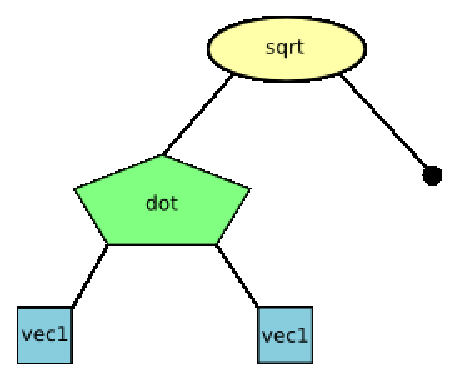
\includegraphics[scale=0.5]{Images/DotMathTreeExample.eps}
\caption{\label{figure:DotFunMathTree}The MathTree for the Assignment command in the magnitude
GmatFunction}
\end{center}
\end{figure}

Note that while the dot GmatFunction has been identified as a needed element for the Assignment
line, there is not yet an instance of a GmatFunction object that is associated with the dot
function, even though the MathTree shown in Figure~\ref{figure:DotFunMathTree} has a FunctionRunner
MathNode that requires it.  This issue will be resolved shortly.

The Sandbox takes this new Function Control Sequence, and checks it for the presence of a
GmatFunction by walking through the list of commands in the control sequence.  When it checks the
Assignment command, it finds that there is a function dependency, and that the associated function
does not exist in the Global Object Store.  Since all function types except for GmatFunctions must
be created before they can be used, the Sandbox assumes that the needed function is a GmatFunction
and asks the Moderator to create an unnamed GmatFunction\footnote{The GmatFunction is unnamed so
that it will not be passed to the configuration.}.

The Moderator calls the Factory Manager to create the function, and returns the pointer of the new
function to the Sandbox.  The Sandbox then sets its name to be ``dot'' and adds it to the Global
Object Store.  The Sandbox also performs the preinitialization steps described above: it sets the
solar system pointer and transient force vector pointer on the function, sets any pointers
referenced by the function, and calls the function's Initialize() method.  Finally, the Sandbox
calls the Moderator to locate the function file for the GmatFunction and sets the path to the file,
completing this piece of the initialization.  The Sandbox then passes the function pointer to the
Assignment command, which passes it, in turn, into the FunctionRunner node.  At this point, the
Sandbox can continue initializing the Assignment command.  The GmatFunction data is set as
shown in Table~\ref{table:GMFdotFunctionDiscovered}.

\begin{center}
\tablecaption{\label{table:GMFdotFunctionDiscovered}GmatFunction Status after Creating the dot
Function}
\tablefirsthead{
\hline
%\color{blue}
\multicolumn{1}{|p{0.9in}|}{\textbf{Function}} &
\multicolumn{1}{m{0.65in}|}{\textbf{Function Object Store}} &
\multicolumn{1}{m{0.62in}|}{\textbf{Global Object Store}} &
\multicolumn{1}{m{0.83in}|}{\textbf{inputs}} &
\multicolumn{1}{m{0.75in}|}{\textbf{outputs}} &
\multicolumn{1}{m{0.8in}|}{\textbf{Function Control Sequence}} &
\multicolumn{1}{m{0.7in}|}{\textbf{Call Stack}} \\
%\color{black}
\hline
}
\tablehead{
\hline
\multicolumn{7}{|r|}{\begin{small}\textit{Continued from previous page}\end{small}}\\
\hline
%\color{blue}
\multicolumn{1}{|m{0.9in}|}{\textbf{Function}} &
\multicolumn{1}{m{0.65in}|}{\textbf{Function Object Store}} &
\multicolumn{1}{m{0.62in}|}{\textbf{Global Object Store}} &
\multicolumn{1}{m{0.83in}|}{\textbf{inputs}} &
\multicolumn{1}{m{0.75in}|}{\textbf{outputs}} &
\multicolumn{1}{m{0.8in}|}{\textbf{Function Control Sequence}} &
\multicolumn{1}{m{0.7in}|}{\textbf{Call Stack}} \\
%\color{black}
\hline
}
\tabletail{
\hline
\multicolumn{7}{|r|}{\begin{small}\textit{Continued on next page}\end{small}}\\ \hline
}
\tablelasttail{\hline}
\begin{supertabular}{|p{0.9in}|p{0.65in}|p{0.62in}|p{0.83in}|p{0.75in}|p{0.8in}|p{0.7in}|}
\hline
\begin{small}LoadCartState\end{small} &
\begin{small}empty\end{small} &
\begin{small}Set\end{small} &
\begin{small}'Sat'->NULL\end{small} &
\begin{small}'rv'->NULL

'vv'->NULL

'r'->NULL

'v'->NULL\end{small} &
\begin{small}Create

Create

Assignment

Assignment

Assignment

Assignment

Assignment

Assignment

CallFunction

CallFunction\end{small} &
\begin{small}empty\end{small}\\
\hline
\begin{small}cross\end{small} & \begin{small}empty\end{small} &
\begin{small}NULL\end{small} & \begin{small}empty\end{small} &
\begin{small}empty\end{small} & \begin{small}empty\end{small} &
\begin{small}empty\end{small}\\
\hline
\begin{small}magnitude\end{small} & \begin{small}empty\end{small} & \begin{small}Set\end{small} &
\begin{small}'vec1'->NULL\end{small} & \begin{small}'val'->NULL\end{small} &
\begin{small}
Create

Assignment 
\end{small} & \begin{small}empty\end{small}\\
\hline
\begin{small}dot\end{small} & \begin{small}empty\end{small} &
\begin{small}NULL\end{small} & \begin{small}empty\end{small} &
\begin{small}empty\end{small} & \begin{small}empty\end{small} &
\begin{small}empty\end{small}\\
\hline
\end{supertabular}
\end{center}

Recall that we are at the point in the initialization where the Sandbox is checking the Function
Control Sequence for the magnitude GmatFunction for internal function calls.  The Sandbox found the
dot function as an internal dependency, and built the corresponding GmatFunction.  The final step
performed by the Sandbox at this point is to build the Function Control Sequence for the dot
command.  The text of the dot file looks like this:

\begin{quote}
\begin{verbatim}
function [val] = dot(vec1, vec2)

% This function takes two 3-vectors in a GMAT array and
% constructs their dot product
Create Variable val
val = vec1(1,1) * vec2(1,1) + vec1(2,1) * vec2(2,1) +...
      vec1(3,1) * vec2(3,1);
\end{verbatim} 
\end{quote}

The Sandbox calls the Moderator::InterpretGmatFunction() method to build the control sequence for
the dot function.  Upon return, the function attribute table has the contents shown in
Table~\ref{table:GMFdotFunctionBuilt}.

\begin{center}
\tablecaption{\label{table:GMFdotFunctionBuilt}GmatFunction Status after Interpreting the dot
Function}
\tablefirsthead{
\hline
%\color{blue}
\multicolumn{1}{|p{0.9in}|}{\textbf{Function}} &
\multicolumn{1}{m{0.65in}|}{\textbf{Function Object Store}} &
\multicolumn{1}{m{0.62in}|}{\textbf{Global Object Store}} &
\multicolumn{1}{m{0.83in}|}{\textbf{inputs}} &
\multicolumn{1}{m{0.75in}|}{\textbf{outputs}} &
\multicolumn{1}{m{0.8in}|}{\textbf{Function Control Sequence}} &
\multicolumn{1}{m{0.7in}|}{\textbf{Call Stack}} \\
%\color{black}
\hline
}
\tablehead{
\hline
\multicolumn{7}{|r|}{\begin{small}\textit{Continued from previous page}\end{small}}\\
\hline
%\color{blue}
\multicolumn{1}{|m{0.9in}|}{\textbf{Function}} &
\multicolumn{1}{m{0.65in}|}{\textbf{Function Object Store}} &
\multicolumn{1}{m{0.62in}|}{\textbf{Global Object Store}} &
\multicolumn{1}{m{0.83in}|}{\textbf{inputs}} &
\multicolumn{1}{m{0.75in}|}{\textbf{outputs}} &
\multicolumn{1}{m{0.8in}|}{\textbf{Function Control Sequence}} &
\multicolumn{1}{m{0.7in}|}{\textbf{Call Stack}} \\
%\color{black}
\hline
}
\tabletail{
\hline
\multicolumn{7}{|r|}{\begin{small}\textit{Continued on next page}\end{small}}\\ \hline
}
\tablelasttail{\hline}
\begin{supertabular}{|p{0.9in}|p{0.65in}|p{0.62in}|p{0.83in}|p{0.75in}|p{0.8in}|p{0.7in}|}
\hline
\begin{small}LoadCartState\end{small} &
\begin{small}empty\end{small} &
\begin{small}Set\end{small} &
\begin{small}'Sat'->NULL\end{small} &
\begin{small}'rv'->NULL

'vv'->NULL

'r'->NULL

'v'->NULL\end{small} &
\begin{small}Create

Create

Assignment

Assignment

Assignment

Assignment

Assignment

Assignment

CallFunction

CallFunction\end{small} &
\begin{small}empty\end{small}\\
\hline
\begin{small}cross\end{small} & \begin{small}empty\end{small} &
\begin{small}NULL\end{small} & \begin{small}empty\end{small} &
\begin{small}empty\end{small} & \begin{small}empty\end{small} &
\begin{small}empty\end{small}\\
\hline
\begin{small}magnitude\end{small} & \begin{small}empty\end{small} & \begin{small}Set\end{small} &
\begin{small}'vec1'->NULL\end{small} & \begin{small}'val'->NULL\end{small} &
\begin{small}
Create

Assignment 
\end{small} & \begin{small}empty\end{small}\\
\hline
\begin{small}dot\end{small} & 
\begin{small}empty\end{small} &
\begin{small}Set\end{small} & 
\begin{small}
'vec1'->NULL

'vec2'->NULL
\end{small} &
\begin{small}
'val'->NULL
\end{small} &
\begin{small}
Create

Assignment
\end{small} &
\begin{small}empty\end{small}\\
\hline
\end{supertabular}
\end{center}

%%% Need to fix this text: %%%%%%%%%%%%%%%%%%%%%%%%%%%%%%%%%%%%%%%%%%%%%%%%%%%%%%%%%%%%%%%%%%%%%%%%%
The Sandbox takes the Function Control Sequence built for the dot function,
and checks it for internal function calls.  There is an Assignment command
in this control sequence that references inline mathematics, but the
corresponding MathTree does not contain any functions. Therefore, the
initialization for the dot function is complete, and the method that built
it returns control to the calling method.

In this case, the calling method is actually the same method that called
the first CallFunction -- the call was a recursive call, because we were
checking the Function Control Sequence for the dot function, which was
called part way through the check of the Function Control Sequence for the
magnitude function.

That call was made for the Assignment command in the magnitude function.
The check for the magnitude Assignment command has now built all of the
functions it needs, so control is returned to the method that was
performing the check on the magnitude function.

Again, the calling method is the method that checks for function calls,
this time for the first CallFunction in the LoadCartState function. 
All of the function references in that CallFunction have been resolved
and initialized, so the function check method moves to the second
CallFunction.  That CallFunction makes a call to the magnitude
function.  All of the internal structures needed to execute the
magnitude function have been built, following the procedures discussed
above.  The check for this CallFunction does detect that there is a
GmatFunction in the call -- a call to the magnitude function.  It then
checks the magnitude GmatFunction, and finds that it has been
initialized, so it proceeds to the next command in the LoadCartState
Function Control Sequence.  Since this second CallFunction was the last
command in that Function Control Sequence, the LoadCartState function
control sequence is now fully initialized and ready to execute.
%%% Fix to here %%%%%%%%%%%%%%%%%%%%%%%%%%%%%%%%%%%%%%%%%%%%%%%%%%%%%%%%%%%%%%%%%%%%%%%%%%%%%%%%%%%%

We have now initialized all of the system except for the cross function.  The Sandbox is partway
through the check on the Mission Control Sequence for function calls -- all of the preceding
GmatFunction initialization was performed to fully initialize the CallFunction command in the
Mission Control Sequence.  The next function encountered in the main script is in the third
Assignment command.  That command was generated by the script line

\begin{quote}
\begin{verbatim}
ev = cross(vv, cross(rv, vv)) / mu - rv / r;
\end{verbatim}
\end{quote}

\noindent When the Sandbox checks that line, it finds that there are two FunctionRunner nodes in the
associated MathTree.  The first of these nodes requires an initialized cross function, so the
Sandbox follows the process described above to build the Function Control Sequence for the cross
function.  Once this first node has been handled by the Sandbox, the function attribute table looks
like Table~\ref{table:GMFcrossFunctionBuilt}.

\begin{center}
\tablecaption{\label{table:GMFcrossFunctionBuilt}GmatFunction Status after Interpreting the cross
Function}
\tablefirsthead{
\hline
%\color{blue}
\multicolumn{1}{|p{0.9in}|}{\textbf{Function}} &
\multicolumn{1}{m{0.65in}|}{\textbf{Function Object Store}} &
\multicolumn{1}{m{0.62in}|}{\textbf{Global Object Store}} &
\multicolumn{1}{m{0.83in}|}{\textbf{inputs}} &
\multicolumn{1}{m{0.75in}|}{\textbf{outputs}} &
\multicolumn{1}{m{0.8in}|}{\textbf{Function Control Sequence}} &
\multicolumn{1}{m{0.7in}|}{\textbf{Call Stack}} \\
%\color{black}
\hline
}
\tablehead{
\hline
\multicolumn{7}{|r|}{\begin{small}\textit{Continued from previous page}\end{small}}\\
\hline
%\color{blue}
\multicolumn{1}{|m{0.9in}|}{\textbf{Function}} &
\multicolumn{1}{m{0.65in}|}{\textbf{Function Object Store}} &
\multicolumn{1}{m{0.62in}|}{\textbf{Global Object Store}} &
\multicolumn{1}{m{0.83in}|}{\textbf{inputs}} &
\multicolumn{1}{m{0.75in}|}{\textbf{outputs}} &
\multicolumn{1}{m{0.8in}|}{\textbf{Function Control Sequence}} &
\multicolumn{1}{m{0.7in}|}{\textbf{Call Stack}} \\
%\color{black}
\hline
}
\tabletail{
\hline
\multicolumn{7}{|r|}{\begin{small}\textit{Continued on next page}\end{small}}\\ \hline
}
\tablelasttail{\hline}
\begin{supertabular}{|p{0.9in}|p{0.65in}|p{0.62in}|p{0.83in}|p{0.75in}|p{0.8in}|p{0.7in}|}
\hline
\begin{small}LoadCartState\end{small} &
\begin{small}empty\end{small} &
\begin{small}Set\end{small} &
\begin{small}'Sat'->NULL\end{small} &
\begin{small}'rv'->NULL

'vv'->NULL

'r'->NULL

'v'->NULL\end{small} &
\begin{small}Create

Create

Assignment

Assignment

Assignment

Assignment

Assignment

Assignment

CallFunction

CallFunction\end{small} &
\begin{small}empty\end{small}\\
\hline
\begin{small}cross\end{small} &  
\begin{small}empty\end{small} &
\begin{small}Set\end{small} & 
\begin{small}
'vec1'->NULL

'vec2'->NULL
\end{small} &
\begin{small}
'vec3'->NULL
\end{small} &
\begin{small}
Create

Assignment

Assignment

Assignment
\end{small} &
\begin{small}empty\end{small}\\
\hline
\begin{small}magnitude\end{small}
& \begin{small}empty\end{small} & \begin{small}Set\end{small} &
\begin{small}'vec1'->NULL\end{small} & \begin{small}'val'->NULL\end{small} &
\begin{small}
Create

Assignment 
\end{small} & \begin{small}empty\end{small}\\
\hline
\begin{small}dot\end{small} & 
\begin{small}empty\end{small} &
\begin{small}Set\end{small} & 
\begin{small}
'vec1'->NULL

'vec2'->NULL
\end{small} &
\begin{small}
'val'->NULL
\end{small} &
\begin{small}
Create

Assignment
\end{small} &
\begin{small}empty\end{small}\\
\hline
\end{supertabular}
\end{center}

The Sandbox then checks the second FunctionRunner node, and finds that it uses a function that has
already been built -- the cross function -- so no further action is necessary for this Assignment
command.  It moves to the next command in the Mission Control Sequence, and finds that that command
-- a CallFunction that uses the magnitude GmatFunction -- is also ready to execute.  This process
continues through all of the remaining commands in the Mission Control Sequence.  All of the
commands and called functions have been initialized, so the commands and functions used in the
Sandbox have now been fully prepared for the mission run.

\paragraph{Additional Notes on Initialization}

\subparagraph{Function and FunctionManager Status Summary}
The scripting in our example generates seven specific places where a FunctionManager interface is
built in order to implement the structure needed to run a GmatFunction. 
Table~\ref{table:GMFFunctionSummary} shows each of these interfaces, along with the string
descriptors that are set in the interface tables for each of these instances.  The actual data
structures that contain the input and output objects are not set during initialization; they are
built the first time the function is called during execution of the Mission Control Sequence.  That
process is described in the execution section of this text.

\begin{center}
\tablecaption{\label{table:GMFFunctionSummary}Summary of the Function Interfaces}
\tablefirsthead{
\hline
%\color{blue}
\multicolumn{1}{|c|}{\multirow{2}{*}{\textbf{Script Line}}} &
\multicolumn{1}{c|}{\multirow{2}{0.5in}{\textbf{Interface Type}}} &
\multicolumn{2}{c|}{\textbf{Function Manager}} &
\multicolumn{3}{c|}{\textbf{Function}} \\
\cline{3-7}
 & &
\multicolumn{1}{c|}{\textit{inputNames}} &
\multicolumn{1}{c|}{\textit{outputNames}} &
\multicolumn{1}{c|}{\textit{name}} &
\multicolumn{1}{c|}{\textit{inputs}} &
\multicolumn{1}{c|}{\textit{outputs}} \\
%\color{black}
\hline
}
\tablehead{
\hline
\multicolumn{7}{|r|}{\begin{small}\textit{Continued from previous page}\end{small}}\\
\hline
%\color{blue}
\multicolumn{1}{|c|}{\multirow{2}{*}{\textbf{Script Line}}} &
\multicolumn{1}{c|}{\multirow{2}{0.5in}{\textbf{Interface Type}}} &
\multicolumn{2}{c|}{\textbf{Function Manager}} &
\multicolumn{3}{c|}{\textbf{Function}} \\
\cline{3-7}
 & &
\multicolumn{1}{c|}{\textit{inputNames}} &
\multicolumn{1}{c|}{\textit{outputNames}} &
\multicolumn{1}{c|}{\textit{name}} &
\multicolumn{1}{c|}{\textit{inputs}} &
\multicolumn{1}{c|}{\textit{outputs}} \\
%\color{black}
\hline
}
\tabletail{
\hline
\multicolumn{7}{|r|}{\begin{small}\textit{Continued on next page}\end{small}}\\ \hline
}
\tablelasttail{\hline}
\begin{supertabular}{|p{0.9in}|p{0.5in}|p{0.62in}|p{0.73in}|p{0.65in}|p{0.8in}|p{0.8in}|}
\hline
\begin{small}
[rv, vv, r, v] = LoadCartState( Sat)
\end{small} &
\begin{small}
Call\-Function
\end{small} &
\begin{small}
'Sat'
\end{small} &
\begin{small}
'rv'

'vv'

'r'

'v'
\end{small} &
\begin{small}
Load\-Cart\-State
\end{small} &
\begin{small}
'Sat'->NULL
\end{small} &
\begin{small}
'rv'->NULL

'vv'-> NULL

'r'->NULL

'v'->NULL
\end{small}\\
\hline
% Second row
\begin{small} % Script line
ev = cross(vv, cross(rv, vv)) / mu - rv / r;
\end{small} &
\begin{small} % Interface Type
Function\-Runner (Two instances)
\end{small} &
\begin{small} % inputNames
'rv'

'vv'
\end{small} &
\begin{small} % outputNames
''
\end{small} &
\begin{small} % name
cross (inner instance)
\end{small} &
\begin{small} % inputs
'vec1'-> NULL

'vec2'-> NULL
\end{small} &
\begin{small} % outputs
'vec3'-> NULL
\end{small}\\
\cline{3-7}
 & &
\begin{small} % inputNames
'vv'

''
\end{small} &
\begin{small} % outputNames
''
\end{small} &
\begin{small} % name
cross (outer instance)
\end{small} &
\begin{small} % inputs
'vec1'-> NULL

'vec2'-> NULL
\end{small} &
\begin{small} % outputs
'vec3'-> NULL
\end{small}\\
\hline
\begin{small} % Script line
[ECC] = magnitude(ev) 
\end{small} &
\begin{small} % Interface Type
Call\-Function
\end{small} &
\begin{small} % inputNames
'ev'
\end{small} &
\begin{small} % outputNames
'ECC'
\end{small} &
\begin{small} % name
magnitude
\end{small} &
\begin{small} % inputs
'vec1'-> NULL
\end{small} &
\begin{small} % outputs
'val'-> NULL
\end{small}\\
\hline
\begin{small} % Script line
[n] = magnitude(nv)
\end{small} &
\begin{small} % Interface Type
Call\-Function
\end{small} &
\begin{small} % inputNames
'nv'
\end{small} &
\begin{small} % outputNames
'n'
\end{small} &
\begin{small} % name
magnitude
\end{small} &
\begin{small} % inputs
'vec1'-> NULL
\end{small} &
\begin{small} % outputs
'val'-> NULL
\end{small}\\
\hline
\begin{small} % Script line
[r] = magnitude(rv)
\end{small} &
\begin{small} % Interface Type
Call\-Function
\end{small} &
\begin{small} % inputNames
'rv'
\end{small} &
\begin{small} % outputNames
'r'
\end{small} &
\begin{small} % name
magnitude
\end{small} &
\begin{small} % inputs
'vec1'-> NULL
\end{small} &
\begin{small} % outputs
'val'-> NULL
\end{small}\\
\hline
\begin{small} % Script line
[v] = magnitude(vv)
\end{small} &
\begin{small} % Interface Type
Call\-Function
\end{small} &
\begin{small} % inputNames
'vv'
\end{small} &
\begin{small} % outputNames
'v'
\end{small} &
\begin{small} % name
magnitude
\end{small} &
\begin{small} % inputs
'vec1'-> NULL
\end{small} &
\begin{small} % outputs
'val'-> NULL
\end{small}\\
\hline
\begin{small} % Script line
val = sqrt(dot( vec1, vec1));
\end{small} &
\begin{small} % Interface Type
Function\-Runner
\end{small} &
\begin{small} % inputNames
'vec1'

'vec1'
\end{small} &
\begin{small} % outputNames
''
\end{small} &
\begin{small} % name
dot
\end{small} &
\begin{small} % inputs
'vec1'-> NULL

'vec2'-> NULL
\end{small} &
\begin{small} % outputs
'val'-> NULL
\end{small}\\
\end{supertabular}
\end{center}

Before we examine execution, a few items should be mentioned about the work performed in the
ScriptInterpreter when the InterpretGmatFunction() method is invoked.

\subparagraph{Details of the  ScriptInterpreter::InterpretGmatFunction() Method} The
Interpreter::Interpret\-GmatFunction()\footnote{While this method is most naturally assigned to the
ScriptInterpreter -- since it is interpreting a text file describing the function -- the method
itself is found in the Interpreter base class.} method is very similar to the
ScriptInterpreter::Interpret() method.  The differences arise in the Interpreter state, the parsing
for the function line in the function file, and the management of the commands created during the
parsing of the function file.

The InterpretGmatFunction() method has this signature:

\begin{quote}
\begin{verbatim}
GmatCommand* Interpreter::InterpretGmatFunction(Function *funct)
\end{verbatim}
\end{quote}

The InterpretGmatFunction() method does not manage state in the same sense as the Interpret()
method.  At the point that the InterpretGmatFunction() method is invoked, there is no longer a sense
of ``object mode'' and ``command mode,'' because every executable line in a GmatFunction file has an
associated command -- in other words, there is no ``object mode'' at this point in the process.
Since there is no sense in tracking state, the Interpreter treats the entire time spent reading and
building the GmatFunction as if it were in Command mode.

When the  InterpretGmatFunction() method is invoked, it takes the Function pointer from the
function's argument list and retrieves the function file name and path from that object.  It opens
the referenced file, and uses the ScriptReadWriter and TextParser helper classes to parse the
function file, one logical block at a time.

The first logical block in a GmatFunction file defines the function, and must start with the
``function'' keyword.  An example of this line can be see in the first line of the cross function in
Listing~5:

\begin{quote}
\begin{verbatim}
function [vec3] = cross(vec1, vec2)
\end{verbatim}
\end{quote}

\noindent If the keyword ``function'' is not encountered as the first element in the command section
of the the first logical block in the file, the method throws an exception stating that the
Interpreter expected a GmatFunction file, but the function definition line is missing.

The remaining elements in this logical block are used to check the function name for a match to the
expected name, and to set the input and output argument lists for the function.  The list contained
in square brackets is sent, one element at a time, into the function as the output elements using
the SetStringParameter() method.  Similarly, the function arguments in parentheses following the
function name generate calls to the SetStringParameter() method, setting the names for the input
arguments.  Thus, for example, the function definition line above for the cross function generates
the following calls into the GmatFunction object that was passed into the InterpretGmatFunction()
method:

\begin{quote}
\begin{verbatim}
// Calls that are made to the cross function.  These are not
// intended to be actual code; they are representative calls.
// The actual code will loop through the argument lists rather
// than perform the linear process shown here.

// Given these values from the TextParser:
//    inputList = {``vec1'', ``vec2''}
//    functionName = ``cross''
//    outputList = {``vec3''}

// First check the name
if (functionName != funct->GetName())
   throw CommandException("The GmatFunction \"" +
      funct->GetName() + "\" in the file \"" + 
      funct->GetStringParameter("Filename") + 
      "\" does not match the function identifier in the file.");

// Next set the input argument(s)\newline
funct->SetStringParameter(INPUTPARAM_ID, inputList[0]);
funct->SetStringParameter(INPUTPARAM_ID, inputList[1]);

// And the output argument(s):
funct->SetStringParameter(OUTPUTPARAM_ID, outputList[0]);
\end{verbatim}
\end{quote}

\noindent (Of course, the exception message should be changed to conform to GMAT's usual message
formats.)  The code in the GmatFunction is built to receive these values, and populate the internal
data structures accordingly.  This, for example, when the line

\begin{quote}
\begin{verbatim}
funct->SetStringParameter(INPUTPARAM_ID, inputList[0]);
\end{verbatim}
\end{quote} 

\noindent is executed, the GmatFunction checks the inputs map and, if the input value is not in the
map, adds it to the map, something like this:

\begin{quote}
\begin{verbatim}
// on this call: SetStringParameter(INPUTPARAM_ID, "vec1"),
// the GmatFunction does this:

if (inputs.find("vec1") == inputs.end())
   inputs["vec1"] = NULL;
else
   throw FunctionException("Invalid operation: an attempt was"
      " made to add an input argument named \"" + "vec1" +
      "\", but an argument with that name already exists.");
\end{verbatim}
\end{quote}

Once the function definition line has been parsed, the process followed to build the Function
Control Sequence begins.  The Function Control Sequence is built using the same process as is
followed for the Mission Control Sequence: the function file is read one logical block at a time,
the command corresponding to that logical block is constructed, and the command is appended to the
control sequence.  The only difference for this phase of initialization is this: when GMAT is
building a Mission Control Sequence, the sequence that receives the new commands is the Mission
Control Sequence associated with the current Sandbox.  For GmatFunction, the control sequence is the
Function Control Sequence associated with the current function.

\subsubsection{GmatFunction Execution}

Once the Mission Control Sequence and all referenced Function Control Sequences have been
initialized, they are ready for execution in the Sandbox.  The Moderator launches execution by
calling the Sandbox::Execute() method.  When this method is called, the Sandbox sets an internal
pointer to the first command in the Mission Control Sequence, and then enters a loop that walks
through the Mission Control Sequence one command at a time.  For each command in the Mission Control
Sequence, the Sandbox performs the following actions:

\begin{enumerate}
\item Check to see if a user interrupt has occurred, and if so, respond to it.
\item Call the Execute() method on the current command.
\item Set the current command pointer to the command returned by calling GetNext() on the command
that just executed.
\item If the new current command pointer is not NULL, loop to step 1; otherwise, the Mission Control
Sequence is finished executing and control returns to the Moderator.
\end{enumerate}

In this section, we will examine the behavior of the execution of the commands that reference
GmatFunctions exclusively.  Readers interested in the general execution of the Mission Control
Sequence are referred to Chapters~\ref{chapter:TopLevel} through~\ref{chapter:Sandbox} and
Chapter~\ref{chapter:Commands} of the GMAT Architectural Specification.

The first command that references a GmatFunction is the command near the top of the While loop which
was generated by this text:

\begin{quote}
\begin{verbatim}
[rv, vv, r, v] = LoadCartState(Sat);
\end{verbatim}
\end{quote}

This script line generates a CallFunction command.  That CallFunction has a FunctionManager that
references the LoadCartState GmatFunction.  The first time Execute() is called for this
CallFunction, these objects have the attributes shown in Table~\ref{table:LCFBeforeFirstExec}.  (For
the CallFunction, only the pointers needed in this discussion are shown in the object stores.  The
example used here does not use any global objects, so just the status of the Global Object Store is
not indicated.)

\begin{center}
\tablecaption{\label{table:LCFBeforeFirstExec}CallFunction Attributes Prior to First Execution}
\tablefirsthead{
\hline
%\color{blue}
\multicolumn{2}{|c|}{\textbf{CallFunction}} &
\multicolumn{3}{c|}{\textbf{FunctionManager}} &
\multicolumn{4}{c|}{\textbf{LoadCartState Function}} \\
\hline
\multicolumn{1}{|m{0.5in}|}{\centering\textit{Sandbox Object Store}} &
\multicolumn{1}{m{0.5in}|}{\centering\textit{Global Object Store}} &
\multicolumn{1}{m{0.4in}|}{\centering\textit{input\-Names}} &
\multicolumn{1}{m{0.4in}|}{\centering\textit{output\-Names}} &
\multicolumn{1}{m{0.5in}|}{\centering\textit{Function Object Store}} &
\multicolumn{1}{c|}{\centering\textit{inputs}} &
\multicolumn{1}{c|}{\centering\textit{outputs}} &
\multicolumn{1}{m{0.5in}|}{\centering\textit{Function Object Store}} &
\multicolumn{1}{m{0.5in}|}{\centering\textit{Global Object Store}} \\
%\color{black}
\hline
}
\tablehead{
\hline
\multicolumn{9}{|r|}{\begin{small}\textit{Continued from previous page}\end{small}}\\
\hline
%\color{blue}
\multicolumn{2}{|c|}{\textbf{CallFunction}} &
\multicolumn{3}{c|}{\textbf{FunctionManager}} &
\multicolumn{4}{c|}{\textbf{LoadCartState Function}} \\
\hline
\multicolumn{1}{|m{0.5in}|}{\centering\textit{Sandbox Object Store}} &
\multicolumn{1}{m{0.5in}|}{\centering\textit{Global Object Store}} &
\multicolumn{1}{m{0.4in}|}{\centering\textit{input\-Names}} &
\multicolumn{1}{m{0.4in}|}{\centering\textit{output\-Names}} &
\multicolumn{1}{m{0.5in}|}{\centering\textit{Function Object Store}} &
\multicolumn{1}{c|}{\centering\textit{inputs}} &
\multicolumn{1}{c|}{\centering\textit{outputs}} &
\multicolumn{1}{m{0.5in}|}{\centering\textit{Function Object Store}} &
\multicolumn{1}{m{0.5in}|}{\centering\textit{Global Object Store}} \\
%\color{black}
\hline
}
\tabletail{
\hline
\multicolumn{9}{|r|}{\begin{small}\textit{Continued on next page}\end{small}}\\ \hline
}
\tablelasttail{\hline}
\begin{supertabular}{|p{0.5in}|p{0.5in}|p{0.4in}|p{0.4in}|p{0.5in}|p{0.68in}|p{0.67in}|p{0.5in}|
p{0.5in}|}
\hline
\begin{small}
Sat

rv

vv

r

v
\end{small} &
\begin{small}
set
\end{small} &
\begin{small}
'Sat'
\end{small} &
\begin{small}
'rv'

'vv'

'r'

'v'
\end{small} &
\begin{small}
empty
\end{small} &
\begin{small}
Sat->NULL
\end{small} &
\begin{small}
rv->NULL

vv->NULL

r->NULL

v->NULL
\end{small} &
\begin{small}
NULL
\end{small} &
\begin{small}
NULL
\end{small} \\
\end{supertabular}
\end{center}

The first time a CallFunction or FunctionRunner is executed, the final piece of initialization is
performed so that all of the data structures used for the execution are set and the Function Control
Sequence is fully initialized.  Subsequent calls into the same CallFunction or FunctionRunner
updates the data used in the function calls by copying the data into the Function Object Store using
the object's assignment operator.  Both of these processes are described below, and illustrated
using our sample functions.

\paragraph{Steps Performed on the First Execution} The first time a CallFunction or FunctionRunner
executes, the following processes are performed:

\begin{enumerate}
\item The CallFunction tells the FunctionManager to build the Function Object Store.  The
FunctionManager performs the following actions in response:
\begin{itemize}
\item First the input arguments are set up:
\begin{itemize}
\item The FunctionManager looks first in the Local Object Store, then in teh Global Object Store,
and finds each input object listed in the inputNames StringArray
\item The input object is cloned, using its Clone() method, and wrapped in an
ObjectWrapper\footnote{For the examples shown here, the function arguuments are all objects, so
they use ObjectWrappers.  Other data types -- real numbers, for example -- use wrappers compatible
with their type.}
\item The Function is queried for the name of the matching input argument
\item The clone is set in the Function Object Store, using the function's argument name as the map
key
\item An ElementWrapper is built for the clone
\item The ElementWrapper is passed to the Function as the input argument
\end{itemize}
\item Then the output arguments are set up:
\begin{itemize}
\item The FunctionManager finds each output object listed in the outputNames StringArray
\item The output object is stored in an ObjectArray for later use
\end{itemize}
\item If this process fails for any input or output object, an exception is thrown and the process
terminates
\item The Function Object Store and Global Object Store are passed into the Function
\end{itemize}
\end{enumerate}

At this point, the objects managed by this CallFunction have the attributes shown in
Table~\ref{table:LCFAfterFOSBuild}.

\begin{center}
\tablecaption{\label{table:LCFAfterFOSBuild}CallFunction Attributes After Building the Function
Object Store}
\tablefirsthead{
\hline
%\color{blue}
\multicolumn{2}{|c|}{\textbf{CallFunction}} &
\multicolumn{3}{c|}{\textbf{FunctionManager}} &
\multicolumn{4}{c|}{\textbf{LoadCartState Function}} \\
\hline
\multicolumn{1}{|m{0.5in}|}{\centering\textit{Sandbox Object Store}} &
\multicolumn{1}{m{0.5in}|}{\centering\textit{Global Object Store}} &
\multicolumn{1}{m{0.4in}|}{\centering\textit{input\-Names}} &
\multicolumn{1}{m{0.4in}|}{\centering\textit{output\-Names}} &
\multicolumn{1}{m{0.5in}|}{\centering\textit{Function Object Store}} &
\multicolumn{1}{c|}{\centering\textit{inputs}} &
\multicolumn{1}{c|}{\centering\textit{outputs}} &
\multicolumn{1}{m{0.5in}|}{\centering\textit{Function Object Store}} &
\multicolumn{1}{m{0.5in}|}{\centering\textit{Global Object Store}} \\
%\color{black}
\hline
}
\tablehead{
\hline
\multicolumn{9}{|r|}{\begin{small}\textit{Continued from previous page}\end{small}}\\
\hline
%\color{blue}
\multicolumn{2}{|c|}{\textbf{CallFunction}} &
\multicolumn{3}{c|}{\textbf{FunctionManager}} &
\multicolumn{4}{c|}{\textbf{LoadCartState Function}} \\
\hline
\multicolumn{1}{|m{0.5in}|}{\centering\textit{Sandbox Object Store}} &
\multicolumn{1}{m{0.5in}|}{\centering\textit{Global Object Store}} &
\multicolumn{1}{m{0.4in}|}{\centering\textit{input\-Names}} &
\multicolumn{1}{m{0.4in}|}{\centering\textit{output\-Names}} &
\multicolumn{1}{m{0.5in}|}{\centering\textit{Function Object Store}} &
\multicolumn{1}{c|}{\centering\textit{inputs}} &
\multicolumn{1}{c|}{\centering\textit{outputs}} &
\multicolumn{1}{m{0.5in}|}{\centering\textit{Function Object Store}} &
\multicolumn{1}{m{0.5in}|}{\centering\textit{Global Object Store}} \\
%\color{black}
\hline
}
\tabletail{
\hline
\multicolumn{9}{|r|}{\begin{small}\textit{Continued on next page}\end{small}}\\ \hline
}
\tablelasttail{\hline}
\begin{supertabular}{|p{0.5in}|p{0.5in}|p{0.4in}|p{0.4in}|p{0.5in}|p{0.68in}|p{0.67in}|p{0.5in}|
p{0.5in}|}
\hline
\begin{small}
Sat

rv

vv

r

v
\end{small} &
\begin{small}
set
\end{small} &
\begin{small}
'Sat'
\end{small} &
\begin{small}
'rv'

'vv'

'r'

'v'
\end{small} &
\begin{small}
'Sat'-> Sat clone
\end{small} &
\begin{small}
Sat-> clone wrapper
\end{small} &
\begin{small}
rv->NULL

vv->NULL

r->NULL

v->NULL
\end{small} &
\begin{small}
set
\end{small} &
\begin{small}
set
\end{small} \\
\end{supertabular}
\end{center}

\begin{enumerate}
\setcounter{enumi}{1}
\item Initialize the Function by calling
Function-{\textgreater}Initialize().  This call makes the Function complete initialization for each
command in the Function Control Sequence.  Each command in the Function Control Sequence
(1)~receives the pointer to the Function Object Store, Global Object Store, transient force vector,
and Solar System, and then (2)~calls the Initialize() method on the command.

\item Execute the Function Control Sequence by walking through the linked list of commands in the
sequence, calling Execute() on each command in the sequence and using the command's GetNext() method
to access the next command that is executed.  Some details are provided below for the behavior of
CallFunction commands and FunctionRunner MathNodes encountered during this process.

Create commands encountered during this execution sequence add their objects to the Function Object
Store.  Global commands add the identified objects to the Global Object Store as well.  At the end
of the execution step, the attributes for the CallFunction example are listed in
Table~\ref{table:LCFAfterCreateCmd}.  Note that the pointers in the outputs attribute have not been
set yet.
\end{enumerate}

\begin{center}
\tablecaption{\label{table:LCFAfterCreateCmd}CallFunction Attributes After Executing the Create
commands}
\tablefirsthead{
\hline
%\color{blue}
\multicolumn{2}{|c|}{\textbf{CallFunction}} &
\multicolumn{3}{c|}{\textbf{FunctionManager}} &
\multicolumn{4}{c|}{\textbf{LoadCartState Function}} \\
\hline
\multicolumn{1}{|m{0.5in}|}{\centering\textit{Sandbox Object Store}} &
\multicolumn{1}{m{0.5in}|}{\centering\textit{Global Object Store}} &
\multicolumn{1}{m{0.4in}|}{\centering\textit{input\-Names}} &
\multicolumn{1}{m{0.4in}|}{\centering\textit{output\-Names}} &
\multicolumn{1}{m{0.5in}|}{\centering\textit{Function Object Store}} &
\multicolumn{1}{c|}{\centering\textit{inputs}} &
\multicolumn{1}{c|}{\centering\textit{outputs}} &
\multicolumn{1}{m{0.5in}|}{\centering\textit{Function Object Store}} &
\multicolumn{1}{m{0.5in}|}{\centering\textit{Global Object Store}} \\
%\color{black}
\hline
}
\tablehead{
\hline
\multicolumn{9}{|r|}{\begin{small}\textit{Continued from previous page}\end{small}}\\
\hline
%\color{blue}
\multicolumn{2}{|c|}{\textbf{CallFunction}} &
\multicolumn{3}{c|}{\textbf{FunctionManager}} &
\multicolumn{4}{c|}{\textbf{LoadCartState Function}} \\
\hline
\multicolumn{1}{|m{0.5in}|}{\centering\textit{Sandbox Object Store}} &
\multicolumn{1}{m{0.5in}|}{\centering\textit{Global Object Store}} &
\multicolumn{1}{m{0.4in}|}{\centering\textit{input\-Names}} &
\multicolumn{1}{m{0.4in}|}{\centering\textit{output\-Names}} &
\multicolumn{1}{m{0.5in}|}{\centering\textit{Function Object Store}} &
\multicolumn{1}{c|}{\centering\textit{inputs}} &
\multicolumn{1}{c|}{\centering\textit{outputs}} &
\multicolumn{1}{m{0.5in}|}{\centering\textit{Function Object Store}} &
\multicolumn{1}{m{0.5in}|}{\centering\textit{Global Object Store}} \\
%\color{black}
\hline
}
\tabletail{
\hline
\multicolumn{9}{|r|}{\begin{small}\textit{Continued on next page}\end{small}}\\ \hline
}
\tablelasttail{\hline}
\begin{supertabular}{|p{0.5in}|p{0.5in}|p{0.4in}|p{0.4in}|p{0.5in}|p{0.68in}|p{0.67in}|p{0.5in}|
p{0.5in}|}
\hline
\begin{small}
Sat

rv

vv

r

v
\end{small} &
\begin{small}
set
\end{small} &
\begin{small}
'Sat'
\end{small} &
\begin{small}
'rv'

'vv'

'r'

'v'
\end{small} &
\begin{small}
'Sat'-> Sat clone

'rv'->rv

'vv'->vv

'r'->r

'v'->v

\end{small} &
\begin{small}
Sat-> clone wrapper
\end{small} &
\begin{small}
rv->NULL

vv->NULL

r->NULL

v->NULL
\end{small} &
\begin{small}
set
\end{small} &
\begin{small}
set
\end{small} \\
\end{supertabular}
\end{center}

\begin{enumerate}
\setcounter{enumi}{3}
\item Retrieve the output data generated from the execution, and use it to set data in the output
arguments that were stored in step 1.  The output arguments are retrieved through a call to

\begin{quote}
\begin{verbatim}
ElementWrapper* Function::GetOutputArgument(Integer argNumber)
\end{verbatim}
\end{quote}

\noindent which finds the output argument at the indicated location and returns it

\item Reset the Function Control Sequence so it is ready for subsequent calls to this function.  The
final state of the function attributes is shown in Table~\ref{table:LCFAfterExecOne}.
\end{enumerate}

\begin{center}
\tablecaption{\label{table:LCFAfterExecOne}CallFunction Attributes After Execution}
\tablefirsthead{
\hline
%\color{blue}
\multicolumn{2}{|c|}{\textbf{CallFunction}} &
\multicolumn{3}{c|}{\textbf{FunctionManager}} &
\multicolumn{4}{c|}{\textbf{LoadCartState Function}} \\
\hline
\multicolumn{1}{|m{0.5in}|}{\centering\textit{Sandbox Object Store}} &
\multicolumn{1}{m{0.5in}|}{\centering\textit{Global Object Store}} &
\multicolumn{1}{m{0.4in}|}{\centering\textit{input\-Names}} &
\multicolumn{1}{m{0.4in}|}{\centering\textit{output\-Names}} &
\multicolumn{1}{m{0.5in}|}{\centering\textit{Function Object Store}} &
\multicolumn{1}{c|}{\centering\textit{inputs}} &
\multicolumn{1}{c|}{\centering\textit{outputs}} &
\multicolumn{1}{m{0.5in}|}{\centering\textit{Function Object Store}} &
\multicolumn{1}{m{0.5in}|}{\centering\textit{Global Object Store}} \\
%\color{black}
\hline
}
\tablehead{
\hline
\multicolumn{9}{|r|}{\begin{small}\textit{Continued from previous page}\end{small}}\\
\hline
%\color{blue}
\multicolumn{2}{|c|}{\textbf{CallFunction}} &
\multicolumn{3}{c|}{\textbf{FunctionManager}} &
\multicolumn{4}{c|}{\textbf{LoadCartState Function}} \\
\hline
\multicolumn{1}{|m{0.5in}|}{\centering\textit{Sandbox Object Store}} &
\multicolumn{1}{m{0.5in}|}{\centering\textit{Global Object Store}} &
\multicolumn{1}{m{0.4in}|}{\centering\textit{input\-Names}} &
\multicolumn{1}{m{0.4in}|}{\centering\textit{output\-Names}} &
\multicolumn{1}{m{0.5in}|}{\centering\textit{Function Object Store}} &
\multicolumn{1}{c|}{\centering\textit{inputs}} &
\multicolumn{1}{c|}{\centering\textit{outputs}} &
\multicolumn{1}{m{0.5in}|}{\centering\textit{Function Object Store}} &
\multicolumn{1}{m{0.5in}|}{\centering\textit{Global Object Store}} \\
%\color{black}
\hline
}
\tabletail{
\hline
\multicolumn{9}{|r|}{\begin{small}\textit{Continued on next page}\end{small}}\\ \hline
}
\tablelasttail{\hline}
\begin{supertabular}{|p{0.5in}|p{0.5in}|p{0.4in}|p{0.4in}|p{0.5in}|p{0.68in}|p{0.67in}|p{0.5in}|
p{0.5in}|}
\hline
\begin{small}
Sat

rv

vv

r

v
\end{small} &
\begin{small}
set
\end{small} &
\begin{small}
'Sat'
\end{small} &
\begin{small}
'rv'

'vv'

'r'

'v'
\end{small} &
\begin{small}
'Sat'-> Sat clone

'rv'->rv

'vv'->vv

'r'->r

'v'->v
\end{small} &
\begin{small}
Sat-> clone wrapper
\end{small} &
\begin{small}
rv->rv

vv->vv

r->r

v->v
\end{small} &
\begin{small}
NULL
\end{small} &
\begin{small}
set
\end{small} \\
\end{supertabular}
\end{center}

\paragraph{Steps Performed on the Subsequent Executions}  Subsequent calls into a CallFunction or
FunctionRunner that has executed once have a simplified first step, because the structures in the
FunctionManager are initialized in the first call.  Subsequent calls follow the following procedure:

\begin{enumerate}
\item The CallFunction tells the FunctionManager to refresh the Function Object Store.  The
FunctionManager performs the following actions in response:
\begin{itemize}
\item The input arguments are updated using the assignment operator to set the clones equal to the
original objects.
\item The Function Object Store is passed into the Function.
\end{itemize}

\noindent At this point, the objects managed by this CallFunction have the attributes shown in
Table~\ref{table:LCFAfterExecTwo}.
\end{enumerate}

\begin{center}
\tablecaption{\label{table:LCFAfterExecTwo}CallFunction Attributes After Execution}
\tablefirsthead{
\hline
%\color{blue}
\multicolumn{2}{|c|}{\textbf{CallFunction}} &
\multicolumn{3}{c|}{\textbf{FunctionManager}} &
\multicolumn{4}{c|}{\textbf{LoadCartState Function}} \\
\hline
\multicolumn{1}{|m{0.5in}|}{\centering\textit{Sandbox Object Store}} &
\multicolumn{1}{m{0.5in}|}{\centering\textit{Global Object Store}} &
\multicolumn{1}{m{0.4in}|}{\centering\textit{input\-Names}} &
\multicolumn{1}{m{0.4in}|}{\centering\textit{output\-Names}} &
\multicolumn{1}{m{0.5in}|}{\centering\textit{Function Object Store}} &
\multicolumn{1}{c|}{\centering\textit{inputs}} &
\multicolumn{1}{c|}{\centering\textit{outputs}} &
\multicolumn{1}{m{0.5in}|}{\centering\textit{Function Object Store}} &
\multicolumn{1}{m{0.5in}|}{\centering\textit{Global Object Store}} \\
%\color{black}
\hline
}
\tablehead{
\hline
\multicolumn{9}{|r|}{\begin{small}\textit{Continued from previous page}\end{small}}\\
\hline
%\color{blue}
\multicolumn{2}{|c|}{\textbf{CallFunction}} &
\multicolumn{3}{c|}{\textbf{FunctionManager}} &
\multicolumn{4}{c|}{\textbf{LoadCartState Function}} \\
\hline
\multicolumn{1}{|m{0.5in}|}{\centering\textit{Sandbox Object Store}} &
\multicolumn{1}{m{0.5in}|}{\centering\textit{Global Object Store}} &
\multicolumn{1}{m{0.4in}|}{\centering\textit{input\-Names}} &
\multicolumn{1}{m{0.4in}|}{\centering\textit{output\-Names}} &
\multicolumn{1}{m{0.5in}|}{\centering\textit{Function Object Store}} &
\multicolumn{1}{c|}{\centering\textit{inputs}} &
\multicolumn{1}{c|}{\centering\textit{outputs}} &
\multicolumn{1}{m{0.5in}|}{\centering\textit{Function Object Store}} &
\multicolumn{1}{m{0.5in}|}{\centering\textit{Global Object Store}} \\
%\color{black}
\hline
}
\tabletail{
\hline
\multicolumn{9}{|r|}{\begin{small}\textit{Continued on next page}\end{small}}\\ \hline
}
\tablelasttail{\hline}
\begin{supertabular}{|p{0.5in}|p{0.5in}|p{0.4in}|p{0.4in}|p{0.5in}|p{0.68in}|p{0.67in}|p{0.5in}|
p{0.5in}|}
\hline
\begin{small}
Sat

rv

vv

r

v
\end{small} &
\begin{small}
set
\end{small} &
\begin{small}
'Sat'
\end{small} &
\begin{small}
'rv'

'vv'

'r'

'v'
\end{small} &
\begin{small}
'Sat'-> Sat clone
\end{small} &
\begin{small}
Sat-> clone wrapper
\end{small} &
\begin{small}
rv->NULL

vv->NULL

r->NULL

v->NULL
\end{small} &
\begin{small}
set
\end{small} &
\begin{small}
set
\end{small} \\
\end{supertabular}
\end{center}

\begin{enumerate}
\setcounter{enumi}{1}
\item Initialize the Function by calling Function-{\textgreater}Initialize().  This call makes the
Function complete initialization for each command in the Function Control Sequence.  Each command in
the Function Control Sequence (1)~receives the pointer to the Function Object Store, Global Object
Store, transient force vector, and Solar System, and then (2)~calls the Initialize() method on the
command.  (This repetition of step 2 is required because the same function can be called from
multiple locations, with different input objects, so the object pointers in the Function Control
Sequence have to be refreshed each time a function is entered.)
\item Execute the Function Control Sequence by walking through the linked list of commands in the
sequence, calling Execute() on each command in the sequence and using the command's GetNext() method
to access the next command that is executed.
\item Retrieve the output data generated from the execution, and use it to set data in the output
arguments.
\item Reset the Function Control Sequence so it is ready for subsequent calls to this function.
\end{enumerate}

\paragraph{Functions within Functions}  GmatFunctions can call other GmatFunctions, either in a
nested manner, or by calling recursively into the same function.  When a GmatFunction detects that
it is about to call into a GmatFunction in this manner, it needs to preserve the current state of
the function data so that, upon return from the nested call, the function can resume execution. 
This preservation of function data is accomplished using a call stack, implemented as the
GmatFunction::\-objectStack data member.

An example of the use of the call stack can be seen in the example script that we've been working
through.  The first function call, made to the LoadCartState function, uses a CallFunction in the
Mission Control Sequence.  When the Sandbox calls this function, the steps outlined in the previous
section are performed, initializing and setting the Function Object Store and Function Control
Sequence, and then calling the Execute method on each command in the Function Control Sequence to
run the function.  The use of the call stack can be seen when we examine the details of this
process, as we will do in the following paragraphs.

When the Sandbox receives a message to execute the Mission Control Sequence, it sets its state to
``RUNNING'' and sets the current command pointer to the first command in the Mission Control
Sequence.  For our example, that means the current pointer start out pointing to the While command
generated by this line of script:

\begin{quote}
\begin{verbatim}
While Sat.ElapsedDays {\textless} 1
\end{verbatim}
\end{quote}

\noindent The command is executed, and control returned to the Sandbox.  The Sandbox then calls the
GetNext() method to determine the next command to execute.  The command pointer returned from that
call points back to the While command again, because the While command is a branch command.  The
Sandbox polls for a user interrupt, and then calls the Execute() method on the While command again. 
The While command begins the execution of the commands inside of the While loop by calling its
ExecuteBranch() method.  That call executes the first command in the while loop,

\begin{quote}
\begin{verbatim}
Propagate Prop(Sat)
\end{verbatim}
\end{quote}

\noindent which advances the spacecraft one step and returns control to the While command.  The
While command then calls GetNext() on the Propagate command that just executed, and sets its loop
command pointer to the returned value -- in this case, a pointer to the CallFunction command
generated by this line:

\begin{quote}
\begin{verbatim}
[rv, vv, r, v] = LoadCartState(Sat);
\end{verbatim}
\end{quote}

\noindent The While command then returns control to the Sandbox.  The Sandbox calls GetNext() on the
While command, and receives, again, a pointer back to the While command, since the While command is
running the commands in the while loop.  The Sandbox polls for interrupts, and then calls Execute()
on the While command, which calls ExecuteBranch(), which, in turn, calls Execute() on the
CallFunction command.  The CallFunction command and FunctionManager have completed initialization
of the GmatFunction as described above, and the CallFunction has made a call into the
FunctionManager::\-Execute() method to run the function. The following discussion picks up at that
point.  I'll refer to this long sequence of calls as the ``Sandbox call chain'' for the rest of this
section -- in other words, the Sandbox call chain is the sequence

\begin{quote}
\begin{verbatim}
Sandbox::Execute() --> While::Execute()
                   --> While::ExecuteBranch()
                   --> CallFunction::Execute()
                   --> FunctionManager::Execute()
\end{verbatim}
\end{quote}

The function that is executing at this point is the LoadCartState GmatFunction, which has the
Function Control Sequence, Function Object Store, and call stack shown in
Table~\ref{table:FunSubfunStart}.  The functions called during execution of this function are also
listed in this table, along with their attributes. The pointer in the FCS column shows the next
command that will be executed; for example, the first Create command in the LoadCartState will be
executed at the point where we resume discussion of the actual process in the next paragraph.

\begin{center}
\tablecaption{\label{table:FunSubfunStart}Attributes of the LoadCartState GmatFunction and
Subfunctions}
\tablefirsthead{
\hline
%\color{blue}
\multicolumn{3}{|c|}{\textbf{LoadCartState}} &
\multicolumn{3}{c|}{\textbf{magnitude}} &
\multicolumn{3}{c|}{\textbf{dot}} \\
\hline
\multicolumn{1}{|m{0.75in}|}{\centering\textit{FCS}} &
\multicolumn{1}{m{0.45in}|}{\centering\textit{FOS}} &
\multicolumn{1}{m{0.45in}|}{\centering\textit{Call Stack}} &
\multicolumn{1}{m{0.69in}|}{\centering\textit{FCS}} &
\multicolumn{1}{m{0.45in}|}{\centering\textit{FOS}} &
\multicolumn{1}{m{0.45in}|}{\centering\textit{Call Stack}} &
\multicolumn{1}{m{0.69in}|}{\centering\textit{FCS}} &
\multicolumn{1}{m{0.45in}|}{\centering\textit{FOS}} &
\multicolumn{1}{m{0.45in}|}{\centering\textit{Call Stack}} \\
%\color{black}
\hline
}
\tablehead{
\hline
\multicolumn{9}{|r|}{\begin{small}\textit{Continued from previous page}\end{small}}\\
\hline
%\color{blue}
\multicolumn{3}{|c|}{\textbf{LoadCartState}} &
\multicolumn{3}{c|}{\textbf{magnitude}} &
\multicolumn{3}{c|}{\textbf{dot}} \\
\hline
\multicolumn{1}{|m{0.75in}|}{\centering\textit{FCS}} &
\multicolumn{1}{m{0.45in}|}{\centering\textit{FOS}} &
\multicolumn{1}{m{0.45in}|}{\centering\textit{Call Stack}} &
\multicolumn{1}{m{0.69in}|}{\centering\textit{FCS}} &
\multicolumn{1}{m{0.45in}|}{\centering\textit{FOS}} &
\multicolumn{1}{m{0.45in}|}{\centering\textit{Call Stack}} &
\multicolumn{1}{m{0.69in}|}{\centering\textit{FCS}} &
\multicolumn{1}{m{0.45in}|}{\centering\textit{FOS}} &
\multicolumn{1}{m{0.45in}|}{\centering\textit{Call Stack}} \\
%\color{black}
\hline
}
\tabletail{
\hline
\multicolumn{9}{|r|}{\begin{small}\textit{Continued on next page}\end{small}}\\ \hline
}
\tablelasttail{\hline}
\begin{supertabular}{|p{0.75in}|p{0.45in}|p{0.45in}|p{0.69in}|p{0.45in}|p{0.45in}|p{0.69in}|
p{0.44in}|p{0.44in}|}
\hline
\begin{small}
>Create

Create

Assignment

Assignment

Assignment

Assignment

Assignment

Assignment

CallFunction

CallFunction
\end{small} &
\begin{small}
Sat clone
\end{small} &
\begin{small}
empty
\end{small} &
\begin{small}
Create

Assignment
\end{small} &
\begin{small}
NULL
\end{small} &
\begin{small}
empty
\end{small} &
\begin{small}
Create

Assignment
\end{small} &
\begin{small}
NULL
\end{small} &
\begin{small}
empty
\end{small} \\
\end{supertabular}
\end{center}

The first call on the Sandbox call chain at this point executes the Create command

\begin{quote}
\begin{verbatim}
Create Variable r v
\end{verbatim}
\end{quote}

placing the variables r and v into the function object store, as is shown in
Table\ref{table:FunSubfunCreate1}.

\begin{center}
\tablecaption{\label{table:FunSubfunCreate1}Attributes of the LoadCartState GmatFunction After the
Executing the First Create Command}
\tablefirsthead{
\hline
%\color{blue}
\multicolumn{3}{|c|}{\textbf{LoadCartState}} &
\multicolumn{3}{c|}{\textbf{magnitude}} &
\multicolumn{3}{c|}{\textbf{dot}} \\
\hline
\multicolumn{1}{|m{0.75in}|}{\centering\textit{FCS}} &
\multicolumn{1}{m{0.45in}|}{\centering\textit{FOS}} &
\multicolumn{1}{m{0.45in}|}{\centering\textit{Call Stack}} &
\multicolumn{1}{m{0.69in}|}{\centering\textit{FCS}} &
\multicolumn{1}{m{0.45in}|}{\centering\textit{FOS}} &
\multicolumn{1}{m{0.45in}|}{\centering\textit{Call Stack}} &
\multicolumn{1}{m{0.69in}|}{\centering\textit{FCS}} &
\multicolumn{1}{m{0.45in}|}{\centering\textit{FOS}} &
\multicolumn{1}{m{0.45in}|}{\centering\textit{Call Stack}} \\
%\color{black}
\hline
}
\tablehead{
\hline
\multicolumn{9}{|r|}{\begin{small}\textit{Continued from previous page}\end{small}}\\
\hline
%\color{blue}
\multicolumn{3}{|c|}{\textbf{LoadCartState}} &
\multicolumn{3}{c|}{\textbf{magnitude}} &
\multicolumn{3}{c|}{\textbf{dot}} \\
\hline
\multicolumn{1}{|m{0.75in}|}{\centering\textit{FCS}} &
\multicolumn{1}{m{0.45in}|}{\centering\textit{FOS}} &
\multicolumn{1}{m{0.45in}|}{\centering\textit{Call Stack}} &
\multicolumn{1}{m{0.69in}|}{\centering\textit{FCS}} &
\multicolumn{1}{m{0.45in}|}{\centering\textit{FOS}} &
\multicolumn{1}{m{0.45in}|}{\centering\textit{Call Stack}} &
\multicolumn{1}{m{0.69in}|}{\centering\textit{FCS}} &
\multicolumn{1}{m{0.45in}|}{\centering\textit{FOS}} &
\multicolumn{1}{m{0.45in}|}{\centering\textit{Call Stack}} \\
%\color{black}
\hline
}
\tabletail{
\hline
\multicolumn{9}{|r|}{\begin{small}\textit{Continued on next page}\end{small}}\\ \hline
}
\tablelasttail{\hline}
\begin{supertabular}{|p{0.75in}|p{0.45in}|p{0.45in}|p{0.69in}|p{0.45in}|p{0.45in}|p{0.69in}|
p{0.44in}|p{0.44in}|}
\hline
\begin{small}
Create

>Create

Assignment

Assignment

Assignment

Assignment

Assignment

Assignment

CallFunction

CallFunction
\end{small} &
\begin{small}
Sat clone

r

v
\end{small} &
\begin{small}
empty
\end{small} &
\begin{small}
Create

Assignment
\end{small} &
\begin{small}
NULL
\end{small} &
\begin{small}
empty
\end{small} &
\begin{small}
Create

Assignment
\end{small} &
\begin{small}
NULL
\end{small} &
\begin{small}
empty
\end{small} \\
\end{supertabular}
\end{center}

The next call executes the second Create command

\begin{quote}\begin{verbatim}

Create Array rv[3,1] vv[3,1]
\end{verbatim}
\end{quote}

\noindent adding the rv and vv arrays to the Function Object Store.  The next six calls execute the
six assignment commands that are used to set the elements of the rv and vv arrays:

\begin{quote}
\begin{verbatim}
rv(1,1) = Sat.X;
rv(1,2) = Sat.Y;
rv(1,3) = Sat.Z;
vv(1,1) = Sat.VX;
vv(1,2) = Sat.VY;
vv(1,3) = Sat.VZ;
\end{verbatim} \end{quote}

Once all of these commands have executed, the attributes contain the data shown in
Table~\ref{table:FunSubfunSixAssigns}, the next command to be executed is the first CallFunction
command, and the function is ready to call the first nested function.

\begin{center}
\tablecaption{\label{table:FunSubfunSixAssigns}Attributes of the LoadCartState Function After the
Executing the Six Assignment Commands}
\tablefirsthead{
\hline
%\color{blue}
\multicolumn{3}{|c|}{\textbf{LoadCartState}} &
\multicolumn{3}{c|}{\textbf{magnitude}} &
\multicolumn{3}{c|}{\textbf{dot}} \\
\hline
\multicolumn{1}{|m{0.75in}|}{\centering\textit{FCS}} &
\multicolumn{1}{m{0.45in}|}{\centering\textit{FOS}} &
\multicolumn{1}{m{0.45in}|}{\centering\textit{Call Stack}} &
\multicolumn{1}{m{0.69in}|}{\centering\textit{FCS}} &
\multicolumn{1}{m{0.45in}|}{\centering\textit{FOS}} &
\multicolumn{1}{m{0.45in}|}{\centering\textit{Call Stack}} &
\multicolumn{1}{m{0.69in}|}{\centering\textit{FCS}} &
\multicolumn{1}{m{0.45in}|}{\centering\textit{FOS}} &
\multicolumn{1}{m{0.45in}|}{\centering\textit{Call Stack}} \\
%\color{black}
\hline
}
\tablehead{
\hline
\multicolumn{9}{|r|}{\begin{small}\textit{Continued from previous page}\end{small}}\\
\hline
%\color{blue}
\multicolumn{3}{|c|}{\textbf{LoadCartState}} &
\multicolumn{3}{c|}{\textbf{magnitude}} &
\multicolumn{3}{c|}{\textbf{dot}} \\
\hline
\multicolumn{1}{|m{0.75in}|}{\centering\textit{FCS}} &
\multicolumn{1}{m{0.45in}|}{\centering\textit{FOS}} &
\multicolumn{1}{m{0.45in}|}{\centering\textit{Call Stack}} &
\multicolumn{1}{m{0.69in}|}{\centering\textit{FCS}} &
\multicolumn{1}{m{0.45in}|}{\centering\textit{FOS}} &
\multicolumn{1}{m{0.45in}|}{\centering\textit{Call Stack}} &
\multicolumn{1}{m{0.69in}|}{\centering\textit{FCS}} &
\multicolumn{1}{m{0.45in}|}{\centering\textit{FOS}} &
\multicolumn{1}{m{0.45in}|}{\centering\textit{Call Stack}} \\
%\color{black}
\hline
}
\tabletail{
\hline
\multicolumn{9}{|r|}{\begin{small}\textit{Continued on next page}\end{small}}\\ \hline
}
\tablelasttail{\hline}
\begin{supertabular}{|p{0.75in}|p{0.45in}|p{0.45in}|p{0.69in}|p{0.45in}|p{0.45in}|p{0.69in}|
p{0.44in}|p{0.44in}|}
\hline
\begin{small}
Create

Create

Assignment

Assignment

Assignment

Assignment

Assignment

Assignment

>CallFunction

CallFunction
\end{small} &
\begin{small}
Sat clone

r

v

rv

vv
\end{small} &
\begin{small}
empty
\end{small} &
\begin{small}
Create

Assignment
\end{small} &
\begin{small}
NULL
\end{small} &
\begin{small}
empty
\end{small} &
\begin{small}
Create

Assignment
\end{small} &
\begin{small}
NULL
\end{small} &
\begin{small}
empty
\end{small} \\
\end{supertabular}
\end{center}

\noindent The CallFunction that is about to be invoked was generated from the script line

\begin{quote}
\begin{verbatim}
[r] = magnitude(rv);
\end{verbatim}
\end{quote}

Whenever the Sandbox call chain invokes a command, the following actions occur in the
FunctionManager\-::Execute() method:

\begin{enumerate}
\item The FunctionManager::Execute() method checks to see if the command that needs to be executed
makes a function call.  If it does:
\begin{itemize}
\item\label{enum:SetNestedRunExecutingFlag}  A flag is set indicating that a nested function is
being run. (This flag is used to prevent repetition of the following bullets when the
FunctionManager::Execute() method is reentered after polling for a user interrupt.)
\item\label{enum:MakeFOSClone} The Function Object Store is cloned.
\item The Function Object Store is placed on the call stack.
\item The nested function (or functions, if more than one function call is made) is initialized. 
The clone of the Function Object Store made in step~\ref{enum:MakeFOSClone} is used as the Local 
Object Map that supplies the arguments that are set in the new Function Object Store, which is then
passed to the nested function during this initialization.
\end{itemize}
\item The Execute() method is called for the command.
\item The GetNext() method is called for the command.  If the pointer returned from this call is
NULL, the flag set in step~\ref{enum:SetNestedRunExecutingFlag} is cleared.
\item Control is returned to the caller so that interrupt polling can occur.
\end{enumerate}

\noindent Once this process is started, calls from the Sandbox call chain into the
FunctionManager::Execute() method as the result of polling for user interrupts skip the first step.

For the CallFunction command under discussion here, the attribute table shown in
Table~\ref{table:FunSubfunCall1Init} describe the internal state of the data immediately following
the initialization in step one.

\begin{center}
\tablecaption{\label{table:FunSubfunCall1Init}The LoadCartState Function after Initializing the
First CallFunction}
\tablefirsthead{
\hline
%\color{blue}
\multicolumn{3}{|c|}{\textbf{LoadCartState}} &
\multicolumn{3}{c|}{\textbf{magnitude}} &
\multicolumn{3}{c|}{\textbf{dot}} \\
\hline
\multicolumn{1}{|m{0.75in}|}{\centering\textit{FCS}} &
\multicolumn{1}{m{0.45in}|}{\centering\textit{FOS}} &
\multicolumn{1}{m{0.45in}|}{\centering\textit{Call Stack}} &
\multicolumn{1}{m{0.69in}|}{\centering\textit{FCS}} &
\multicolumn{1}{m{0.45in}|}{\centering\textit{FOS}} &
\multicolumn{1}{m{0.45in}|}{\centering\textit{Call Stack}} &
\multicolumn{1}{m{0.69in}|}{\centering\textit{FCS}} &
\multicolumn{1}{m{0.45in}|}{\centering\textit{FOS}} &
\multicolumn{1}{m{0.45in}|}{\centering\textit{Call Stack}} \\
%\color{black}
\hline
}
\tablehead{
\hline
\multicolumn{9}{|r|}{\begin{small}\textit{Continued from previous page}\end{small}}\\
\hline
%\color{blue}
\multicolumn{3}{|c|}{\textbf{LoadCartState}} &
\multicolumn{3}{c|}{\textbf{magnitude}} &
\multicolumn{3}{c|}{\textbf{dot}} \\
\hline
\multicolumn{1}{|m{0.75in}|}{\centering\textit{FCS}} &
\multicolumn{1}{m{0.45in}|}{\centering\textit{FOS}} &
\multicolumn{1}{m{0.45in}|}{\centering\textit{Call Stack}} &
\multicolumn{1}{m{0.69in}|}{\centering\textit{FCS}} &
\multicolumn{1}{m{0.45in}|}{\centering\textit{FOS}} &
\multicolumn{1}{m{0.45in}|}{\centering\textit{Call Stack}} &
\multicolumn{1}{m{0.69in}|}{\centering\textit{FCS}} &
\multicolumn{1}{m{0.45in}|}{\centering\textit{FOS}} &
\multicolumn{1}{m{0.45in}|}{\centering\textit{Call Stack}} \\
%\color{black}
\hline
}
\tabletail{
\hline
\multicolumn{9}{|r|}{\begin{small}\textit{Continued on next page}\end{small}}\\ \hline
}
\tablelasttail{\hline}
\begin{supertabular}{|p{0.75in}|p{0.45in}|p{0.45in}|p{0.69in}|p{0.45in}|p{0.45in}|p{0.69in}|
p{0.44in}|p{0.44in}|}
\hline
\begin{small}
Create

Create

Assignment

Assignment

Assignment

Assignment

Assignment

Assignment

>CallFunction

CallFunction
\end{small} &
\begin{small}
Clones of:

Sat clone

r

v

rv

vv
\end{small} &
\begin{small}
Original FOS:

Sat clone

r

v

rv

vv
\end{small} &
\begin{small}
>Create

Assignment
\end{small} &
\begin{small}
'vec1'-> clone of vv clone
\end{small} &
\begin{small}
empty
\end{small} &
\begin{small}
Create

Assignment
\end{small} &
\begin{small}
NULL
\end{small} &
\begin{small}
empty
\end{small} \\
\end{supertabular}
\end{center}

The magnitude GmatFunction is now ready to be run through the LoadCartState function.  The next call
through the Sandbox call chain invokes a call to the magnitude function's Create() command, which
builds a variable named val.  Table~\ref{table:FunSubfunCall1cmd1} shows the attributes after
running this command.

\begin{center}
\tablecaption{\label{table:FunSubfunCall1cmd1}Attributes of the Function After Running the First
magnitude Command}
\tablefirsthead{
\hline
%\color{blue}
\multicolumn{3}{|c|}{\textbf{LoadCartState}} &
\multicolumn{3}{c|}{\textbf{magnitude}} &
\multicolumn{3}{c|}{\textbf{dot}} \\
\hline
\multicolumn{1}{|m{0.75in}|}{\centering\textit{FCS}} &
\multicolumn{1}{m{0.45in}|}{\centering\textit{FOS}} &
\multicolumn{1}{m{0.45in}|}{\centering\textit{Call Stack}} &
\multicolumn{1}{m{0.69in}|}{\centering\textit{FCS}} &
\multicolumn{1}{m{0.45in}|}{\centering\textit{FOS}} &
\multicolumn{1}{m{0.45in}|}{\centering\textit{Call Stack}} &
\multicolumn{1}{m{0.69in}|}{\centering\textit{FCS}} &
\multicolumn{1}{m{0.45in}|}{\centering\textit{FOS}} &
\multicolumn{1}{m{0.45in}|}{\centering\textit{Call Stack}} \\
%\color{black}
\hline
}
\tablehead{
\hline
\multicolumn{9}{|r|}{\begin{small}\textit{Continued from previous page}\end{small}}\\
\hline
%\color{blue}
\multicolumn{3}{|c|}{\textbf{LoadCartState}} &
\multicolumn{3}{c|}{\textbf{magnitude}} &
\multicolumn{3}{c|}{\textbf{dot}} \\
\hline
\multicolumn{1}{|m{0.75in}|}{\centering\textit{FCS}} &
\multicolumn{1}{m{0.45in}|}{\centering\textit{FOS}} &
\multicolumn{1}{m{0.45in}|}{\centering\textit{Call Stack}} &
\multicolumn{1}{m{0.69in}|}{\centering\textit{FCS}} &
\multicolumn{1}{m{0.45in}|}{\centering\textit{FOS}} &
\multicolumn{1}{m{0.45in}|}{\centering\textit{Call Stack}} &
\multicolumn{1}{m{0.69in}|}{\centering\textit{FCS}} &
\multicolumn{1}{m{0.45in}|}{\centering\textit{FOS}} &
\multicolumn{1}{m{0.45in}|}{\centering\textit{Call Stack}} \\
%\color{black}
\hline
}
\tabletail{
\hline
\multicolumn{9}{|r|}{\begin{small}\textit{Continued on next page}\end{small}}\\ \hline
}
\tablelasttail{\hline}
\begin{supertabular}{|p{0.75in}|p{0.45in}|p{0.45in}|p{0.69in}|p{0.45in}|p{0.45in}|p{0.69in}|
p{0.44in}|p{0.44in}|}
\hline
\begin{small}
Create

Create

Assignment

Assignment

Assignment

Assignment

Assignment

Assignment

>CallFunction

CallFunction
\end{small} &
\begin{small}
Clones of:

Sat clone

r

v

rv

vv
\end{small} &
\begin{small}
Original FOS:

Sat clone

r

v

rv

vv
\end{small} &
\begin{small}
Create

>Assignment
\end{small} &
\begin{small}
'vec1'-> clone of vv clone

val
\end{small} &
\begin{small}
empty
\end{small} &
\begin{small}
Create

Assignment
\end{small} &
\begin{small}
NULL
\end{small} &
\begin{small}
empty
\end{small} \\
\end{supertabular}
\end{center}

The next call through the Sandbox call chain invokes the magnitude function's Assignment command,
built off of this line of script:

\begin{quote}
\begin{verbatim}
val = sqrt(dot(vec1, vec1));
\end{verbatim}
\end{quote}

\noindent The right side of this equation generates a MathTree.  One node of that MathTree is a
FunctionRunner, constructed to run the dot GmatFunction.  Hence the check performed by the
FunctionManager that is running the magnitude function detects that there is a nested function call
in its Assignment command.  Accordingly, when it is time to evaluate the MathTree, the controlling
FunctionManager passes a pointer to itself, through the Assignment command, into the MathTree, which
passes that pointer to each FunctionRunner node in the tree.  Then when the MathTree makes the call
to evaluate the FunctionRunner node, the FunctionRunner starts by calling the controlling
FunctionManager::\-PushToStack() method, which clones its local Function Object Store, places the
original on its call stack, and build the Function Object Store for the nested function.  It then
sets the clone as the Function Object Store for the FunctionManager inside of the FunctionRunner,
and calls that FunctionManager's Evaluate() method.  The Evaluate method starts by initializing the
function, using the newly cloned Function Object Store as the source for the objects needed for
initialization.  The resulting attributes are shown in Table~\ref{table:FunSubfunCall1FunRunPrep}.

\begin{center}
\tablecaption{\label{table:FunSubfunCall1FunRunPrep}LoadCartState Attributes After Running the First
magnitude Command}
\tablefirsthead{
\hline
%\color{blue}
\multicolumn{3}{|c|}{\textbf{LoadCartState}} &
\multicolumn{3}{c|}{\textbf{magnitude}} &
\multicolumn{3}{c|}{\textbf{dot}} \\
\hline
\multicolumn{1}{|m{0.75in}|}{\centering\textit{FCS}} &
\multicolumn{1}{m{0.45in}|}{\centering\textit{FOS}} &
\multicolumn{1}{m{0.45in}|}{\centering\textit{Call Stack}} &
\multicolumn{1}{m{0.69in}|}{\centering\textit{FCS}} &
\multicolumn{1}{m{0.45in}|}{\centering\textit{FOS}} &
\multicolumn{1}{m{0.45in}|}{\centering\textit{Call Stack}} &
\multicolumn{1}{m{0.69in}|}{\centering\textit{FCS}} &
\multicolumn{1}{m{0.45in}|}{\centering\textit{FOS}} &
\multicolumn{1}{m{0.45in}|}{\centering\textit{Call Stack}} \\
%\color{black}
\hline
}
\tablehead{
\hline
\multicolumn{9}{|r|}{\begin{small}\textit{Continued from previous page}\end{small}}\\
\hline
%\color{blue}
\multicolumn{3}{|c|}{\textbf{LoadCartState}} &
\multicolumn{3}{c|}{\textbf{magnitude}} &
\multicolumn{3}{c|}{\textbf{dot}} \\
\hline
\multicolumn{1}{|m{0.75in}|}{\centering\textit{FCS}} &
\multicolumn{1}{m{0.45in}|}{\centering\textit{FOS}} &
\multicolumn{1}{m{0.45in}|}{\centering\textit{Call Stack}} &
\multicolumn{1}{m{0.69in}|}{\centering\textit{FCS}} &
\multicolumn{1}{m{0.45in}|}{\centering\textit{FOS}} &
\multicolumn{1}{m{0.45in}|}{\centering\textit{Call Stack}} &
\multicolumn{1}{m{0.69in}|}{\centering\textit{FCS}} &
\multicolumn{1}{m{0.45in}|}{\centering\textit{FOS}} &
\multicolumn{1}{m{0.45in}|}{\centering\textit{Call Stack}} \\
%\color{black}
\hline
}
\tabletail{
\hline
\multicolumn{9}{|r|}{\begin{small}\textit{Continued on next page}\end{small}}\\ \hline
}
\tablelasttail{\hline}
\begin{supertabular}{|p{0.75in}|p{0.45in}|p{0.45in}|p{0.69in}|p{0.45in}|p{0.45in}|p{0.69in}|
p{0.44in}|p{0.44in}|}
\hline
\begin{small}
Create

Create

Assignment

Assignment

Assignment

Assignment

Assignment

Assignment

>CallFunction

CallFunction
\end{small} &
\begin{small}
Clones of:

Sat clone

r

v

rv

vv
\end{small} &
\begin{small}
Original FOS:

Sat clone

r

v

rv

vv
\end{small} &
\begin{small}
Create

>Assignment
\end{small} &
\begin{small}
Clones of: 
'vec1'-> clone of vv clone

val
\end{small} &
\begin{small}
Original FOS:

'vec1'-> clone of vv clone

val
\end{small} &
\begin{small}
>Create

Assignment
\end{small} &
\begin{small}
'vec1'-> clone of clone of vv clone

'vec2'-> clone of clone of vv clone
\end{small} &
\begin{small}
empty
\end{small} \\
\end{supertabular}
\end{center}

The dot function can now be run.  This execution is made by calling the Evaluate() method on the
FunctionRunner.  In turn, the FunctionRunner executes the function.  Fortunately, this function does
not call another.  Upon completion of the execution of the dot function, the attributes have the
values shown in Table~\ref{table:FunSubfunCall1FunRundotDone}.

\begin{center}
\tablecaption{\label{table:FunSubfunCall1FunRundotDone}LoadCartState Attributes After Evaluating the
dot Function in the magnitude Function}
\tablefirsthead{
\hline
%\color{blue}
\multicolumn{3}{|c|}{\textbf{LoadCartState}} &
\multicolumn{3}{c|}{\textbf{magnitude}} &
\multicolumn{3}{c|}{\textbf{dot}} \\
\hline
\multicolumn{1}{|m{0.75in}|}{\centering\textit{FCS}} &
\multicolumn{1}{m{0.45in}|}{\centering\textit{FOS}} &
\multicolumn{1}{m{0.45in}|}{\centering\textit{Call Stack}} &
\multicolumn{1}{m{0.69in}|}{\centering\textit{FCS}} &
\multicolumn{1}{m{0.45in}|}{\centering\textit{FOS}} &
\multicolumn{1}{m{0.45in}|}{\centering\textit{Call Stack}} &
\multicolumn{1}{m{0.69in}|}{\centering\textit{FCS}} &
\multicolumn{1}{m{0.45in}|}{\centering\textit{FOS}} &
\multicolumn{1}{m{0.45in}|}{\centering\textit{Call Stack}} \\
%\color{black}
\hline
}
\tablehead{
\hline
\multicolumn{9}{|r|}{\begin{small}\textit{Continued from previous page}\end{small}}\\
\hline
%\color{blue}
\multicolumn{3}{|c|}{\textbf{LoadCartState}} &
\multicolumn{3}{c|}{\textbf{magnitude}} &
\multicolumn{3}{c|}{\textbf{dot}} \\
\hline
\multicolumn{1}{|m{0.75in}|}{\centering\textit{FCS}} &
\multicolumn{1}{m{0.45in}|}{\centering\textit{FOS}} &
\multicolumn{1}{m{0.45in}|}{\centering\textit{Call Stack}} &
\multicolumn{1}{m{0.69in}|}{\centering\textit{FCS}} &
\multicolumn{1}{m{0.45in}|}{\centering\textit{FOS}} &
\multicolumn{1}{m{0.45in}|}{\centering\textit{Call Stack}} &
\multicolumn{1}{m{0.69in}|}{\centering\textit{FCS}} &
\multicolumn{1}{m{0.45in}|}{\centering\textit{FOS}} &
\multicolumn{1}{m{0.45in}|}{\centering\textit{Call Stack}} \\
%\color{black}
\hline
}
\tabletail{
\hline
\multicolumn{9}{|r|}{\begin{small}\textit{Continued on next page}\end{small}}\\ \hline
}
\tablelasttail{\hline}
\begin{supertabular}{|p{0.75in}|p{0.45in}|p{0.45in}|p{0.69in}|p{0.45in}|p{0.45in}|p{0.69in}|
p{0.44in}|p{0.44in}|}
\hline
\begin{small}
Create

Create

Assignment

Assignment

Assignment

Assignment

Assignment

Assignment

>CallFunction

CallFunction
\end{small} &
\begin{small}
Clones of:

Sat clone

r

v

rv

vv
\end{small} &
\begin{small}
Original FOS:

Sat clone

r

v

rv

vv
\end{small} &
\begin{small}
Create

>Assignment
\end{small} &
\begin{small}
Clones of: 
'vec1'-> clone of vv clone

val
\end{small} &
\begin{small}
Original FOS:

'vec1'-> clone of vv clone

val
\end{small} &
\begin{small}
Create

Assignment
\end{small} &
\begin{small}
'vec1'-> clone of clone of vv clone

'vec2'-> clone of clone of vv clone

val
\end{small} &
\begin{small}
empty
\end{small} \\
\end{supertabular}
\end{center}

At this point we can start unwinding the call stack.  The Function Object Store for the dot function
includes a Variable, val, that has the scalar product of the vv Array with itself.  Once the dot
function has completed execution, the FunctionManager retrieves this value, and saves it so that it
can be passed to the MathTree as the result of the Evaluate() call on the FunctionRunner node.  The
FunctionManger then finalizes the dot function, clearing the Function Object Store pointer in the
dot function.  The FunctionRunner then calls the controlling FunctionManager's PopFromStack()
method, which deletes the cloned call stack and restores the Function Object Store that was on the
call stack.  The MathTree completes its evaluation, retrieving the values obtained from the dot
function, and using that value to build the resultant needed by the Assignment command that contains
the MathTree.  The attributes at this point are shown in
Table~\ref{table:FunSubfunCall1FunRunmagDone}.

\begin{center}
\tablecaption{\label{table:FunSubfunCall1FunRunmagDone}LoadCartState Attributes After Evaluating the
magnitude Assignment Command}
\tablefirsthead{
\hline
%\color{blue}
\multicolumn{3}{|c|}{\textbf{LoadCartState}} &
\multicolumn{3}{c|}{\textbf{magnitude}} &
\multicolumn{3}{c|}{\textbf{dot}} \\
\hline
\multicolumn{1}{|m{0.75in}|}{\centering\textit{FCS}} &
\multicolumn{1}{m{0.45in}|}{\centering\textit{FOS}} &
\multicolumn{1}{m{0.45in}|}{\centering\textit{Call Stack}} &
\multicolumn{1}{m{0.69in}|}{\centering\textit{FCS}} &
\multicolumn{1}{m{0.45in}|}{\centering\textit{FOS}} &
\multicolumn{1}{m{0.45in}|}{\centering\textit{Call Stack}} &
\multicolumn{1}{m{0.69in}|}{\centering\textit{FCS}} &
\multicolumn{1}{m{0.45in}|}{\centering\textit{FOS}} &
\multicolumn{1}{m{0.45in}|}{\centering\textit{Call Stack}} \\
%\color{black}
\hline
}
\tablehead{
\hline
\multicolumn{9}{|r|}{\begin{small}\textit{Continued from previous page}\end{small}}\\
\hline
%\color{blue}
\multicolumn{3}{|c|}{\textbf{LoadCartState}} &
\multicolumn{3}{c|}{\textbf{magnitude}} &
\multicolumn{3}{c|}{\textbf{dot}} \\
\hline
\multicolumn{1}{|m{0.75in}|}{\centering\textit{FCS}} &
\multicolumn{1}{m{0.45in}|}{\centering\textit{FOS}} &
\multicolumn{1}{m{0.45in}|}{\centering\textit{Call Stack}} &
\multicolumn{1}{m{0.69in}|}{\centering\textit{FCS}} &
\multicolumn{1}{m{0.45in}|}{\centering\textit{FOS}} &
\multicolumn{1}{m{0.45in}|}{\centering\textit{Call Stack}} &
\multicolumn{1}{m{0.69in}|}{\centering\textit{FCS}} &
\multicolumn{1}{m{0.45in}|}{\centering\textit{FOS}} &
\multicolumn{1}{m{0.45in}|}{\centering\textit{Call Stack}} \\
%\color{black}
\hline
}
\tabletail{
\hline
\multicolumn{9}{|r|}{\begin{small}\textit{Continued on next page}\end{small}}\\ \hline
}
\tablelasttail{\hline}
\begin{supertabular}{|p{0.75in}|p{0.45in}|p{0.45in}|p{0.69in}|p{0.45in}|p{0.45in}|p{0.69in}|
p{0.44in}|p{0.44in}|}
\hline
\begin{small}
Create

Create

Assignment

Assignment

Assignment

Assignment

Assignment

Assignment

>CallFunction

CallFunction
\end{small} &
\begin{small}
Clones of:

Sat clone

r

v

rv

vv
\end{small} &
\begin{small}
Original FOS:

Sat clone

r

v

rv

vv
\end{small} &
\begin{small}
Create

Assignment
\end{small} &
\begin{small}
'vec1'-> clone of vv clone

val
\end{small} &
\begin{small}
empty\end{small} &
\begin{small}
Create

Assignment
\end{small} &
\begin{small}
NULL
\end{small} &
\begin{small}
empty
\end{small} \\
\end{supertabular}
\end{center}

%%% Try to make clearer %%%%%%%%%%%%%%%%%%%%%%%%%%%%%%%%%%%%%%%%%%%%%%%%%%%%%%%%%%%%%%%%%%%%%%%%%%%%

The Assignment command that called into the dot function used the results of that function to set
the value of the val Variable in the magnitude function's Function Object Store.  That Assignment
command was the last command in the magnitude function's Function Control Sequence, so the call to
the magnitude function made from the LoadCartState function has completed execution.  The
FunctionManager for the LoadCartState function retrieves the output argument -- in this case, the
val Variable -- from the magnitude function.  It then deletes the cloned function object store, pops
the Function Object Store off of the call stack, locates the object set to contain the output --
that is, the r Variable -- in this Function Object Store, and calls the assignment operator to set
these two objects equal.  That process is followed for all of the output arguments in the function
call, and then the FunctionManager clears the magnitude function, completing the execution of the
CallFunction command.  These steps result in the attributes tabulated in
Table~\ref{table:FunSubfunCall1FunRunmagClear}.
%%% To here %%%%%%%%%%%%%%%%%%%%%%%%%%%%%%%%%%%%%%%%%%%%%%%%%%%%%%%%%%%%%%%%%%%%%%%%%%%%%%%%%%%%%%%%

\begin{center}
\tablecaption{\label{table:FunSubfunCall1FunRunmagClear}LoadCartState Attributes After Clearing the
magnitude Function}
\tablefirsthead{
\hline
%\color{blue}
\multicolumn{3}{|c|}{\textbf{LoadCartState}} &
\multicolumn{3}{c|}{\textbf{magnitude}} &
\multicolumn{3}{c|}{\textbf{dot}} \\
\hline
\multicolumn{1}{|m{0.75in}|}{\centering\textit{FCS}} &
\multicolumn{1}{m{0.45in}|}{\centering\textit{FOS}} &
\multicolumn{1}{m{0.45in}|}{\centering\textit{Call Stack}} &
\multicolumn{1}{m{0.69in}|}{\centering\textit{FCS}} &
\multicolumn{1}{m{0.45in}|}{\centering\textit{FOS}} &
\multicolumn{1}{m{0.45in}|}{\centering\textit{Call Stack}} &
\multicolumn{1}{m{0.69in}|}{\centering\textit{FCS}} &
\multicolumn{1}{m{0.45in}|}{\centering\textit{FOS}} &
\multicolumn{1}{m{0.45in}|}{\centering\textit{Call Stack}} \\
%\color{black}
\hline
}
\tablehead{
\hline
\multicolumn{9}{|r|}{\begin{small}\textit{Continued from previous page}\end{small}}\\
\hline
%\color{blue}
\multicolumn{3}{|c|}{\textbf{LoadCartState}} &
\multicolumn{3}{c|}{\textbf{magnitude}} &
\multicolumn{3}{c|}{\textbf{dot}} \\
\hline
\multicolumn{1}{|m{0.75in}|}{\centering\textit{FCS}} &
\multicolumn{1}{m{0.45in}|}{\centering\textit{FOS}} &
\multicolumn{1}{m{0.45in}|}{\centering\textit{Call Stack}} &
\multicolumn{1}{m{0.69in}|}{\centering\textit{FCS}} &
\multicolumn{1}{m{0.45in}|}{\centering\textit{FOS}} &
\multicolumn{1}{m{0.45in}|}{\centering\textit{Call Stack}} &
\multicolumn{1}{m{0.69in}|}{\centering\textit{FCS}} &
\multicolumn{1}{m{0.45in}|}{\centering\textit{FOS}} &
\multicolumn{1}{m{0.45in}|}{\centering\textit{Call Stack}} \\
%\color{black}
\hline
}
\tabletail{
\hline
\multicolumn{9}{|r|}{\begin{small}\textit{Continued on next page}\end{small}}\\ \hline
}
\tablelasttail{\hline}
\begin{supertabular}{|p{0.75in}|p{0.45in}|p{0.45in}|p{0.69in}|p{0.45in}|p{0.45in}|p{0.69in}|
p{0.44in}|p{0.44in}|}
\hline
\begin{small}
Create

Create

Assignment

Assignment

Assignment

Assignment

Assignment

Assignment

CallFunction

>CallFunction
\end{small} &
\begin{small}
Sat clone

r

v

rv

vv
\end{small} &
\begin{small}
empty
\end{small} &
\begin{small}
Create

Assignment
\end{small} &
\begin{small}
NULL
\end{small} &
\begin{small}
empty\end{small} &
\begin{small}
Create

Assignment
\end{small} &
\begin{small}
NULL
\end{small} &
\begin{small}
empty
\end{small} \\
\end{supertabular}
\end{center}

This process is repeated for the last CallFunction in the LoadCartState Function Control Sequence,
resulting in calls that set the value of the v Variable in the LoadCartState Function Object Store. 
Once this final CallFunction has been evaluated, the FunctionManager in the Mission Control Sequence
CallFunction command that started this process -- that is, the FunctionManager that is running the
LoadCartState function -- retrieves the output objects, one at a time, and sets the objects in the
Sandbox Object Map referenced by the CallFunction command equal to the objects found in the
LoadCartState Function Object Store using the corresponding assignment operators.  This completes
the LoadCartState function execution, so the CallFunction FunctionManager finalizess the
LoadCartState function, resulting in the attributes shown in
Table~\ref{table:FunSubfunCall1FunRunAllClear}.  The LoadCartState function is now ready for a new
call, should one be encountered later in the mission.

\begin{center}
\tablecaption{\label{table:FunSubfunCall1FunRunAllClear}Attributes after running the LoadCartState
Function}
\tablefirsthead{
\hline
%\color{blue}
\multicolumn{3}{|c|}{\textbf{LoadCartState}} &
\multicolumn{3}{c|}{\textbf{magnitude}} &
\multicolumn{3}{c|}{\textbf{dot}} \\
\hline
\multicolumn{1}{|m{0.75in}|}{\centering\textit{FCS}} &
\multicolumn{1}{m{0.45in}|}{\centering\textit{FOS}} &
\multicolumn{1}{m{0.45in}|}{\centering\textit{Call Stack}} &
\multicolumn{1}{m{0.69in}|}{\centering\textit{FCS}} &
\multicolumn{1}{m{0.45in}|}{\centering\textit{FOS}} &
\multicolumn{1}{m{0.45in}|}{\centering\textit{Call Stack}} &
\multicolumn{1}{m{0.69in}|}{\centering\textit{FCS}} &
\multicolumn{1}{m{0.45in}|}{\centering\textit{FOS}} &
\multicolumn{1}{m{0.45in}|}{\centering\textit{Call Stack}} \\
%\color{black}
\hline
}
\tablehead{
\hline
\multicolumn{9}{|r|}{\begin{small}\textit{Continued from previous page}\end{small}}\\
\hline
%\color{blue}
\multicolumn{3}{|c|}{\textbf{LoadCartState}} &
\multicolumn{3}{c|}{\textbf{magnitude}} &
\multicolumn{3}{c|}{\textbf{dot}} \\
\hline
\multicolumn{1}{|m{0.75in}|}{\centering\textit{FCS}} &
\multicolumn{1}{m{0.45in}|}{\centering\textit{FOS}} &
\multicolumn{1}{m{0.45in}|}{\centering\textit{Call Stack}} &
\multicolumn{1}{m{0.69in}|}{\centering\textit{FCS}} &
\multicolumn{1}{m{0.45in}|}{\centering\textit{FOS}} &
\multicolumn{1}{m{0.45in}|}{\centering\textit{Call Stack}} &
\multicolumn{1}{m{0.69in}|}{\centering\textit{FCS}} &
\multicolumn{1}{m{0.45in}|}{\centering\textit{FOS}} &
\multicolumn{1}{m{0.45in}|}{\centering\textit{Call Stack}} \\
%\color{black}
\hline
}
\tabletail{
\hline
\multicolumn{9}{|r|}{\begin{small}\textit{Continued on next page}\end{small}}\\ \hline
}
\tablelasttail{\hline}
\begin{supertabular}{|p{0.75in}|p{0.45in}|p{0.45in}|p{0.69in}|p{0.45in}|p{0.45in}|p{0.69in}|
p{0.44in}|p{0.44in}|}
\hline
\begin{small}
Create

Create

Assignment

Assignment

Assignment

Assignment

Assignment

Assignment

CallFunction

CallFunction
\end{small} &
\begin{small}
NULL
\end{small} &
\begin{small}
empty
\end{small} &
\begin{small}
Create

Assignment
\end{small} &
\begin{small}
NULL
\end{small} &
\begin{small}
empty\end{small} &
\begin{small}
Create

Assignment
\end{small} &
\begin{small}
NULL
\end{small} &
\begin{small}
empty
\end{small} \\
\end{supertabular}
\end{center}

\subsubsection{Finalization}
The final step in running scripts that use GMAT functions is the cleanup after the function has been
run.  The normal procedure followed in the Sandbox is to call RunComplete() on the Mission Control
Sequence, which gives each command the opportunity to reset itself for a subsequent run.  The
CallFunction and Assignment commands that access GmatFunctions use this call to execute the
RunComplete() method in the Function Control Sequences contained in those functions.

The Sandbox Object Map and Global Object Store are left intact when GMAT finishes a run.  Subsequent
runs in GMAT start by clearing and reloading these object stores.  The preservation of the final
states of the objects in the Sandbox makes it possible to query these objects for final state data
after a run completes execution.

\subsection{Global Data Handling: Another Short Example}
In this section, we will examine another short sample to show how global data is managed in GMAT
when functions are present.  The main script that drives this example is shown here:

\begin{quote}
\begin{verbatim}
Create ImpulsiveBurn globalBurn;
Create Spacecraft globalSat;
Create Variable index;

Create ForceModel fm
fm.PrimaryBodies = {Earth}
Create Propagator prop
prop.FM = fm

Create OpenGLPlot OGLPlot1;
GMAT OGLPlot1.Add = {globalSat, Earth};

Global globalBurn globalSat
Propagate prop(globalSat) {globalSat.Earth.Periapsis}
For index = 1 : 4
  RaiseApogee(index);
  Propagate prop(globalSat) {globalSat.Earth.Periapsis}
EndFor
\end{verbatim} 
\end{quote} 

The function called here, RaiseApogee, applies a maneuver to the spacecraft so that subsequent
propagation moves the spacecraft on different trajectory.  The function is defined like this:

\begin{quote}
\begin{verbatim}
function [] = RaiseApogee(burnSize)

Global globalBurn globalSat
globalBurn.Element1 = burnSize / 10.0;
Maneuver globalBurn(globalSat);
\end{verbatim}
\end{quote}

This function uses two objects that are not defined in the function, and that are also not passed in
using arguments to the function.  These objects are placed in the Sandbox's Global Object Store.  In
the next few pages we will examine this object repository during initialization, execution, and
finalization.

\subsubsection{Globals During Initialization}

At the start of initialization in the Sandbox, the Global Object Store is empty, the Sandbox Object
Map contains the objects from the Configuration, and the Mission Control Sequence has been built
from parsing of the script.  The state of the objects in the Sandbox immediately before the start of
Mission Control Sequence initialization is shown in Table~\ref{table:GlobalExampleStart}.

\begin{center}
\tablecaption{\label{table:GlobalExampleStart}The Objects in the Globals Example at the
Start of Initialization}
\tablefirsthead{
\hline
%\color{blue}
\multicolumn{3}{|c|}{\textbf{Mission Objects}} &
\multicolumn{3}{c|}{\textbf{RaiseApogee Function}} \\
\hline
\multicolumn{1}{|m{0.95in}|}{\centering\textit{Sandbox Object Map}} &
\multicolumn{1}{m{0.95in}|}{\centering\textit{Global Object Store}} &
\multicolumn{1}{m{0.95in}|}{\centering\textit{Mission Control Sequence}} &
\multicolumn{1}{m{0.95in}|}{\centering\textit{Function Object Store}} &
\multicolumn{1}{m{0.95in}|}{\centering\textit{Global Object Map}} &
\multicolumn{1}{m{0.95in}|}{\centering\textit{Function Control Sequence}} \\
%\color{black}
\hline
}
\tablehead{
\hline
\multicolumn{6}{|r|}{\begin{small}\textit{Continued from previous page}\end{small}}\\
\hline
%\color{blue}
\multicolumn{3}{|c|}{\textbf{Mission Objects}} &
\multicolumn{3}{c|}{\textbf{RaiseApogee Function}} \\
\hline
\multicolumn{1}{|m{0.95in}|}{\centering\textit{Sandbox Object Map}} &
\multicolumn{1}{m{0.95in}|}{\centering\textit{Global Object Store}} &
\multicolumn{1}{m{0.95in}|}{\centering\textit{Mission Control Sequence}} &
\multicolumn{1}{m{0.95in}|}{\centering\textit{Function Object Store}} &
\multicolumn{1}{m{0.95in}|}{\centering\textit{Global Object Map}} &
\multicolumn{1}{m{0.95in}|}{\centering\textit{Function Control Sequence}} \\
%\color{black}
\hline
}
\tabletail{
\hline
\multicolumn{6}{|r|}{\begin{small}\textit{Continued on next page}\end{small}}\\
\hline
}
\tablelasttail{\hline}
\begin{supertabular}{|p{0.95in}|p{0.95in}|p{0.95in}|p{0.95in}|p{0.95in}|p{0.95in}|}
\hline
\begin{small}
globalBurn

globalSat

index

fm

prop

EarthMJ2000Eq

EarthMJ2000Ec

EarthFixed

OGLPlot1

RaiseApogee
\end{small} &
\begin{small}
empty
\end{small} &
\begin{small}
Global

Propagate

For

CallFunction

Propagate

EndFor
\end{small} &
\begin{small}
NULL
\end{small} &
\begin{small}
NULL
\end{small} &
\begin{small}
empty
\end{small} \\
\end{supertabular}
\end{center}

The first thing the Sandbox does after initializing the objects in the Sandbox Object Map is to
collect all objects in the Sandbox Object Store that are marked as globals via the isGlobal flag,
and moves those objects into the Global Object Store.  This includes the objects that are
automatically set as global in scope.  Other objects are set as globals using a check box on the
GUI, or using the ``MakeGlobal'' object property in the script file.  For this example, neither case
is met, so the only global objects are the automatic globals -- the Propagator and the
Function found in the script, along with the three coordinate systems that GMAT automatically
creates. Table~\ref{table:GlobalExampleMoved} shows the resulting rearrangement of objects.  Note
that the objects marked by the Global command in the script are not put into the Global Object
Store at this point.  They are moved when the Global command is executed.

\begin{center}
\tablecaption{\label{table:GlobalExampleMoved}The Objects in the Globals Example after moving the
Globals}
\tablefirsthead{
\hline
%\color{blue}
\multicolumn{3}{|c|}{\textbf{Mission Objects}} &
\multicolumn{3}{c|}{\textbf{RaiseApogee Function}} \\
\hline
\multicolumn{1}{|m{0.95in}|}{\centering\textit{Sandbox Object Map}} &
\multicolumn{1}{m{0.95in}|}{\centering\textit{Global Object Store}} &
\multicolumn{1}{m{0.95in}|}{\centering\textit{Mission Control Sequence}} &
\multicolumn{1}{m{0.95in}|}{\centering\textit{Function Object Store}} &
\multicolumn{1}{m{0.95in}|}{\centering\textit{Global Object Map}} &
\multicolumn{1}{m{0.95in}|}{\centering\textit{Function Control Sequence}} \\
%\color{black}
\hline
}
\tablehead{
\hline
\multicolumn{6}{|r|}{\begin{small}\textit{Continued from previous page}\end{small}}\\
\hline
%\color{blue}
\multicolumn{3}{|c|}{\textbf{Mission Objects}} &
\multicolumn{3}{c|}{\textbf{RaiseApogee Function}} \\
\hline
\multicolumn{1}{|m{0.95in}|}{\centering\textit{Sandbox Object Map}} &
\multicolumn{1}{m{0.95in}|}{\centering\textit{Global Object Store}} &
\multicolumn{1}{m{0.95in}|}{\centering\textit{Mission Control Sequence}} &
\multicolumn{1}{m{0.95in}|}{\centering\textit{Function Object Store}} &
\multicolumn{1}{m{0.95in}|}{\centering\textit{Global Object Map}} &
\multicolumn{1}{m{0.95in}|}{\centering\textit{Function Control Sequence}} \\
%\color{black}
\hline
}
\tabletail{
\hline
\multicolumn{6}{|r|}{\begin{small}\textit{Continued on next page}\end{small}}\\
\hline
}
\tablelasttail{\hline}
\begin{supertabular}{|p{0.95in}|p{0.95in}|p{0.95in}|p{0.95in}|p{0.95in}|p{0.95in}|}
\hline
\begin{small}
globalBurn

globalSat

index

fm

OGLPlot1
\end{small} &
\begin{small}
prop

EarthMJ2000Eq

EarthMJ2000Ec

EarthFixed

RaiseApogee
\end{small} &
\begin{small}
Global

Propagate

For

CallFunction

Propagate

EndFor
\end{small} &
\begin{small}
NULL
\end{small} &
\begin{small}
NULL
\end{small} &
\begin{small}
empty
\end{small} \\
\end{supertabular}
\end{center}

\noindent Note that the global objects have been moved from the Sandbox Object Map into the Global
Object Store.  This feature -- glossed over in the earlier discussion -- makes memory management for
the objects at the Sandbox level simple.  When the Sandbox is cleared, all of the objects in the
Sandbox Object Map and the Global Object Store are deleted.

This feature has implications for global objects created inside of functions as well.  If an object
created inside of a function is declared global, either explicitly using a Global command or
implicitly by virtue of its type, the Create or Global command checks the Global Object Store to see
if an object of that name is already stored in it.  If the object already exists in the Global
Object Store, the types of the objects are compared, and if they do not match, an exception is
thrown. Additional discussion of the interplay between the Create command and the Global command are
provided in the design specifications for those commands.

Once the automatic globals have been moved into the Global Object Store, the Sandbox proceeds with
initialization of the commands in the Mission Control Sequence.  This process follows the procedure
described in the preceding sections, so the results are summarized here, with details related to
global objects discussed more completely.

The first command of interest in this discussion is the Global command.  At construction, this
command was given the names of the global objects identified for the command.  These names are
stored in the command for use at execution time.  No action is applied for this command during
initialization.

The next command of interest is the CallFunction command.  When the CallFunction command
initializes, the Global Object Store pointer is passed into the function contained in the
CallFunction -- in this case, the RaiseApogee function.  Then the solar system and transient force
vector pointers are set in the function.  The function is then retrieved by the Sandbox, and passed
to the ScriptInterpreter::InterpretGmatFunction() method, which builds the Function Control
Sequence.  Upon return, the attributes are set as shown in Table~\ref{table:GlobalExampleIGFReturn}.

\begin{center}
\tablecaption{\label{table:GlobalExampleIGFReturn}The Objects in the Globals Example on return from
InterpretGmatFunction}
\tablefirsthead{
\hline
%\color{blue}
\multicolumn{3}{|c|}{\textbf{Mission Objects}} &
\multicolumn{3}{c|}{\textbf{RaiseApogee Function}} \\
\hline
\multicolumn{1}{|m{0.95in}|}{\centering\textit{Sandbox Object Map}} &
\multicolumn{1}{m{0.95in}|}{\centering\textit{Global Object Store}} &
\multicolumn{1}{m{0.95in}|}{\centering\textit{Mission Control Sequence}} &
\multicolumn{1}{m{0.95in}|}{\centering\textit{Function Object Store}} &
\multicolumn{1}{m{0.95in}|}{\centering\textit{Global Object Map}} &
\multicolumn{1}{m{0.95in}|}{\centering\textit{Function Control Sequence}} \\
%\color{black}
\hline
}
\tablehead{
\hline
\multicolumn{6}{|r|}{\begin{small}\textit{Continued from previous page}\end{small}}\\
\hline
%\color{blue}
\multicolumn{3}{|c|}{\textbf{Mission Objects}} &
\multicolumn{3}{c|}{\textbf{RaiseApogee Function}} \\
\hline
\multicolumn{1}{|m{0.95in}|}{\centering\textit{Sandbox Object Map}} &
\multicolumn{1}{m{0.95in}|}{\centering\textit{Global Object Store}} &
\multicolumn{1}{m{0.95in}|}{\centering\textit{Mission Control Sequence}} &
\multicolumn{1}{m{0.95in}|}{\centering\textit{Function Object Store}} &
\multicolumn{1}{m{0.95in}|}{\centering\textit{Global Object Map}} &
\multicolumn{1}{m{0.95in}|}{\centering\textit{Function Control Sequence}} \\
%\color{black}
\hline
}
\tabletail{
\hline
\multicolumn{6}{|r|}{\begin{small}\textit{Continued on next page}\end{small}}\\
\hline
}
\tablelasttail{\hline}
\begin{supertabular}{|p{0.95in}|p{0.95in}|p{0.95in}|p{0.95in}|p{0.95in}|p{0.95in}|}
\hline
\begin{small}
globalBurn

globalSat

index

fm

OGLPlot1
\end{small} &
\begin{small}
prop

EarthMJ2000Eq

EarthMJ2000Ec

EarthFixed

RaiseApogee
\end{small} &
\begin{small}
Global

Propagate

For

CallFunction

Propagate

EndFor
\end{small} &
\begin{small}
NULL
\end{small} &
\begin{small}
set
\end{small} &
\begin{small}
Global

Assignment

Maneuver
\end{small} \\
\end{supertabular}
\end{center}

Like the Mission Control Sequence, the Function Control Sequence contains a Global command.  The
names of the global objects identified for this command are set in the InterpretGmatFunction()
method when the GmatFunction is parsed.  Nothing else happens for the Global command during the
initialization that builds the Function Control Sequence.

The Sandbox continues initializing the commands in the Mission Control Sequence until they are all
initialized, completing the process.

\subsubsection{Globals During Execution}
Next we will examine the behavior of the Global commands during execution of the Mission Control
Sequence.  The first command that is executed in the Mission Control Sequence is the Global command
defined by the line

\begin{quote}
\begin{verbatim}
Global globalBurn globalSat
\end{verbatim}
\end{quote}

\noindent in the Function Control Sequence.  This command contains a list of the global objects,
specified as objects named ``globalBurn'' and ``globalSat''.  When the Global::\-Execute() method is
called, it takes this list and, for each element in the list, performs these actions:

\begin{enumerate}
\item\label{enum:GlobalEnumStart} Check the command's object map (in this case the Sandbox Object
Store) for the named object. 
\item If the object was found:
\begin{enumerate}
\item Check the Global Object Store for an object with the same name.
\item\label{enum:MoveToGlobal} If no such object was found, remove the object from the object map
and set it in the Global Object Store.  Continue at step~\ref{enum:ContinueOrExit}.
\item If the object was found in the Global Object Store, throw an exception stating that an object
was found in the Global Object Store with the same name as one that was being added, and terminate
the run.
\end{enumerate}
\item The object is not in the object map, so the Global command needs to verify that it was set by
another process in the Global Object store.  Looks for the object, and verify that it in the Global
Object Store and that its pointer is not NULL.  If the pointer is NULL, throw an exception and
terminate the run.
\item\label{enum:ContinueOrExit} Get the next name from the list of global objects.  If the list is
finished, exit, otherwise, return to step~\ref{enum:GlobalEnumStart} to process the next global
object.
\end{enumerate}

The Global command in the Mission Control Sequence follows the process shown in
step~\ref{enum:MoveToGlobal}, moving the declared objects into the Global Object store, as shown in
Table~\ref{table:GlobalExampleIGFRunDone}.

\begin{center}
\tablecaption{\label{table:GlobalExampleIGFRunDone}The Objects in the Globals Example after
Executing the Global Command in the Mission Control Sequence}
\tablefirsthead{
\hline
%\color{blue}
\multicolumn{3}{|c|}{\textbf{Mission Objects}} &
\multicolumn{3}{c|}{\textbf{RaiseApogee Function}} \\
\hline
\multicolumn{1}{|m{0.95in}|}{\centering\textit{Sandbox Object Map}} &
\multicolumn{1}{m{0.95in}|}{\centering\textit{Global Object Store}} &
\multicolumn{1}{m{0.95in}|}{\centering\textit{Mission Control Sequence}} &
\multicolumn{1}{m{0.95in}|}{\centering\textit{Function Object Store}} &
\multicolumn{1}{m{0.95in}|}{\centering\textit{Global Object Map}} &
\multicolumn{1}{m{0.95in}|}{\centering\textit{Function Control Sequence}} \\
%\color{black}
\hline
}
\tablehead{
\hline
\multicolumn{6}{|r|}{\begin{small}\textit{Continued from previous page}\end{small}}\\
\hline
%\color{blue}
\multicolumn{3}{|c|}{\textbf{Mission Objects}} &
\multicolumn{3}{c|}{\textbf{RaiseApogee Function}} \\
\hline
\multicolumn{1}{|m{0.95in}|}{\centering\textit{Sandbox Object Map}} &
\multicolumn{1}{m{0.95in}|}{\centering\textit{Global Object Store}} &
\multicolumn{1}{m{0.95in}|}{\centering\textit{Mission Control Sequence}} &
\multicolumn{1}{m{0.95in}|}{\centering\textit{Function Object Store}} &
\multicolumn{1}{m{0.95in}|}{\centering\textit{Global Object Map}} &
\multicolumn{1}{m{0.95in}|}{\centering\textit{Function Control Sequence}} \\
%\color{black}
\hline
}
\tabletail{
\hline
\multicolumn{6}{|r|}{\begin{small}\textit{Continued on next page}\end{small}}\\
\hline
}
\tablelasttail{\hline}
\begin{supertabular}{|p{0.95in}|p{0.95in}|p{0.95in}|p{0.95in}|p{0.95in}|p{0.95in}|}
\hline
\begin{small}
index

fm

OGLPlot1
\end{small} &
\begin{small}
prop

EarthMJ2000Eq

EarthMJ2000Ec

EarthFixed

RaiseApogee

globalBurn

globalSat
\end{small} &
\begin{small}
Global

Propagate

For

CallFunction

Propagate

EndFor
\end{small} &
\begin{small}
NULL
\end{small} &
\begin{small}
set
\end{small} &
\begin{small}
Global

Assignment

Maneuver
\end{small} \\
\end{supertabular}
\end{center}

\noindent Execution of the Global command in the Mission Control Sequence simply verifies that the
global objects are set as specified.

\subsection{Additional Notes and Comments}
This section contains a few items that may need additional notes to fully explain the function
design.

\subsubsection{Search Order for Reference Objects}
Previous builds of GMAT contain a single mapping for reference object names, the Sandbox Object Map.
 The function subsystem design requires the addition of two new mappings between names and object
pointer: the Global Object Store and the Function Object Store.  

In context, a command only has access to two of these three possible mappings.  The Global Object
Store is visible to all commands.  Commands that are part of the Mission Control Sequence also
access the Sandbox Object Map, while commands in a Function Control Sequence access the function's
Function Object Store.  I'll refer to this second mapping -- either the Sandbox Object Map or the
Function Object Store, depending on context -- as the Local Object Store.

It is possible that objects in the Local Object Store have identical names to objects in the Global
Object Store.  As an example, both the dot and cross functions described in the function example in
this document use local objects named vec1 and vec2.  If one of these functions declared vec1 as a
global object, a call to execute that function would move the local vec1 object into the Global
Object Store.  A subsequent call to the other function would result in a case where both the Local
Object Store and the Global Object Store contain an object named vec1, and the commands that use
this object would need a rule that specifies how to resolve the referenced object between these two
object mappings.

The general rule for resolving reference objects for this type of scenario is that local objects
have precedence over global objects.  When reference object pointers are located prior to executing
a command, the Local Object Store is searched first for the named object.  If the Local Object Store
does not contain the reference object, then the Global Object Store is used to resolve the
reference.  If the object is not found there either, an exception is thrown stating that a
referenced object -- with a specified name that is states in the exception message -- was not
available for use by the command.

\subsubsection{Identifying Global Objects using the isGlobal Flag}

The GmatBase base class gains a new attribute as part of the function design.  This attribute is a
boolean data member named isGlobal, which defaults to false in the base class.  The isGlobal
attribute can be accessed using the Get/SetBooleanParameter methods through the script
identifier ``MakeGlobal''.  Thus, in parameter mode, the following scripting:

\begin{quote}
\begin{verbatim}
Create Spacecraft Satellite
Satellite.MakeGlobal = true
\end{verbatim} 
\end{quote} 

\noindent specifies that the Spacecraft named Satellite is a global object, and should be placed in
the Global Object Store when that mapping is populated -- for example, as part of the global object
mapping described in Initialization Step 3 (see section~\ref{section:GlobalObjectManagement}).

The isGlobal flag is used by GMAT's GUI to determine the state of the Global checkbox on resource
panels -- if the isGlobal flag is true, then a call to the Get\-Boolean\-Parameter(\-"MakeGlobal")
method returns true, and the box is checked.  When a user changes the state of the checkbox, that
change is passed to the object using a call to the Set\-Boolean\-Parameter(\-``MakeGlobal'',
newValue) method.

In the Sandbox, the Global command moves local objects into the Global Object Store.  When the
command moves an object, it also toggles the isGlobal flag so that queries made to the object can
identify that the object is globally acessible.  This state data can be used by the Create command
to determine if an object that it manages has been added to the Global Object Store, and therefore
does not need to be resent to an object map.
